\documentclass[11pt,a4paper]{article}

\usepackage[a4paper,top=18mm,bottom=18mm,left=18mm,right=18mm]{geometry}
\usepackage[T1]{fontenc}
\usepackage{lmodern,microtype}
\usepackage{amsmath,amssymb,mathtools,bm}
\usepackage{xcolor,booktabs,tabularx,array,enumitem,multicol,graphicx}
\usepackage{tikz}
\usetikzlibrary{arrows.meta,positioning,calc}
\usepackage[most]{tcolorbox}
\usepackage{fancyhdr,hyperref}
\definecolor{ink}{HTML}{24354B}
\definecolor{accent}{HTML}{135E77}
\definecolor{pale}{HTML}{F1F7F8}
\hypersetup{colorlinks=true,linkcolor=accent,urlcolor=accent,pdfauthor={PHYS4055 revision notes}}
\setlength{\parindent}{0pt}
\setlength{\parskip}{4pt}
\setlength{\emergencystretch}{3em}
\setlist{leftmargin=*,topsep=2pt,itemsep=1pt}
\AtBeginDocument{\color{ink}}
\pagestyle{fancy}
\fancyhf{}
\fancyhead[L]{\footnotesize PHYS4055 \textbar\ Exam Revision}
\fancyhead[R]{\footnotesize 2026 \textbar\ Open-book notes}
\fancyfoot[C]{\footnotesize\thepage}
\renewcommand{\headrulewidth}{0.3pt}
\newcommand{\ket}[1]{\left\lvert #1\right\rangle}
\newcommand{\bra}[1]{\left\langle #1\right\rvert}
\newcommand{\braket}[2]{\left\langle #1\middle\vert #2\right\rangle}
\newcommand{\mel}[3]{\left\langle #1\middle\vert #2\middle\vert #3\right\rangle}
\newcommand{\diff}{\mathrm{d}}
\newcommand{\ii}{\mathrm{i}}
\newcommand{\e}{\mathrm{e}}
\newtcolorbox{methodbox}{colback=pale,colframe=accent!50!white,boxrule=0.4pt,arc=1mm,before skip=5pt,after skip=5pt}
\newtcolorbox{cautionbox}{colback=white,colframe=black!20,boxrule=0.4pt,arc=1mm,before skip=5pt,after skip=5pt}

\usepackage{titlesec}
\geometry{top=18mm,bottom=19mm,left=19mm,right=19mm,headsep=7mm,footskip=9mm}
\hypersetup{
pdftitle={PHYS4055 - Mini-Textbook: Atomic Physics and Quantum Optics},
pdfsubject={A readable four-part course guide with derived formulas and worked examples}
}
\linespread{1.055}
\setlength{\parskip}{3.5pt plus .6pt minus .2pt}
\setlength{\emergencystretch}{3em}
\setlength{\headheight}{14pt}
\setcounter{tocdepth}{1}
\titleformat{\section}{\Large\bfseries\color{accent}}{\thesection}{.6em}{}
\titleformat{\subsection}{\normalsize\bfseries\color{accent}}{\thesubsection}{.5em}{}
\titlespacing*{\section}{0pt}{10pt}{9pt}
\titlespacing*{\subsection}{0pt}{10pt}{4pt}
\renewcommand{\arraystretch}{1.15}
\fancyhead[L]{\footnotesize PHYS4055 \textbar\ Mini-Textbook}
\fancyhead[R]{\footnotesize Physics from principles to applications}
\newtcolorbox{intuition}{
enhanced,breakable,colback=pale,colframe=accent!65!black,
boxrule=.6pt,arc=1mm,before skip=7pt,after skip=7pt,
title={The physical picture},fonttitle=\bfseries}
\newtcolorbox{checkpoint}{
enhanced,breakable,colback=white,colframe=accent!45!black,
boxrule=.45pt,arc=.8mm,before skip=6pt,after skip=6pt,
title={Concept check},fonttitle=\bfseries}
\newtcolorbox{worked}[1]{
enhanced,breakable,colback=pale,colframe=accent,
boxrule=.7pt,arc=1mm,before skip=7pt,after skip=7pt,
title={Worked example: #1},fonttitle=\bfseries}
\newcommand{\unit}[1]{\clearpage\section{#1}}
\newcommand{\unitref}[1]{\vspace{-1mm}
\noindent{\footnotesize\color{gray}
\textbf{Course sources:} #1}\par\vspace{3mm}}
\newcommand{\partmarking}[2]{
\addcontentsline{toc}{part}{Part #1: #2}
}
\begin{document}
\begin{titlepage}
\centering
\vspace*{18mm}
{\color{accent}\Huge\bfseries PHYS4055\par}
\vspace{8mm}
{\LARGE Atomic Physics and Quantum Optics\par}
\vspace{15mm}
{\huge\bfseries A Mini-Textbook\par}
\vspace{4mm}
{\Large From physical ideas to equations and worked examples\par}
\vspace{10mm}
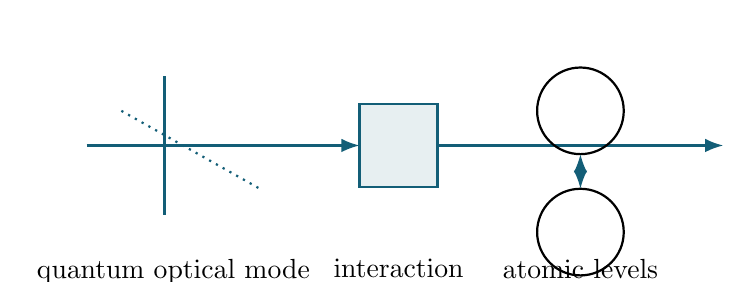
\begin{tikzpicture}[scale=1.1,>=Latex]
\draw[->,thick,accent](-3.7,0)--(-.55,0);
\draw[thick,accent,fill=accent!10](-.55,-.48)rectangle(.35,.48);
\draw[->,thick,accent](.35,0)--(3.65,0);
\draw[accent,very thick](-2.8,-.8)--(-2.8,.8);
\draw[accent,dotted,thick](-3.3,.4)--(-1.7,-.5);
\draw[thick] (2,-1.0) circle(.5);
\draw[thick] (2,0.4) circle(.5);
\draw[<->,accent,thick](2,-.5)--(2,-.1);
\node[below]at(-2.7,-1.2){quantum optical mode};
\node[below]at(2,-1.2){atomic levels};
\node[below]at(-.1,-1.2){interaction};
\end{tikzpicture}
\vspace{11mm}

\begin{minipage}{.88\textwidth}
\begin{methodbox}
\textbf{Four connected parts:}\\
I.\ \ Quantised light, photon statistics and squeezing\\
II.\ Quantum information, open systems and metrology\\
III.\ Atomic wavefunctions, electron coupling and structure\\
IV.\ Spectroscopy, cooling, symmetry tests and atomic clocks
\end{methodbox}
\end{minipage}
\vfill
{\large Course-based revision edition \(\cdot\) November 2026\par}
\vspace{4mm}
{\small Companion to the 15-page overview, tutorial/assignment
worked solutions and 2023--2025 exam answers.\par}
\end{titlepage}

\tableofcontents
\clearpage
\section*{How to use this mini-textbook}
\addcontentsline{toc}{section}{How to use this mini-textbook}
This is a \emph{teaching document} for the full PHYS4055
course, not an abbreviated formula sheet.
Its purpose is to answer three questions:
what is happening physically, why the formula
has its particular form, and how that formula
helps solve an exam problem.
The 15-page overview is designed for fast lookup;
this book is intended to be \emph{read and worked through}.

\subsection*{A suggested route through the material}
The course has four connected parts.
Quantum optics first describes light as quantised
field modes. Applications of optics use those
states, operations and measurements to
communicate, process information and make
sensitive measurements. Atomic physics
introduces electron wavefunctions, angular
momentum, energy-level splitting and transition
matrix elements. Applications of atomic physics
use these ideas in cooling and trapping,
symmetry tests and clocks.

If quantum notation feels unfamiliar, start
with Chapters 1--4 before trying the
applications. If your main difficulty is
angular-momentum coupling, read Chapters
14--16 slowly, including their worked
examples. Later chapters repeatedly
refer back to these ideas.

\subsection*{Mathematical notation, explained}
A ket \(\ket\psi\) is a quantum state vector.
A bra \(\bra\phi\) is its conjugate transpose.
The inner product \(\braket\phi\psi\)
is a complex amplitude and
\(|\braket\phi\psi|^2\) is a probability
when the states are normalised.
A matrix element \(\mel fO i\) asks
how strongly the operator \(O\)
connects initial \(\ket i\) to final
\(\ket f\). A commutator is
\([A,B]=AB-BA\); it measures
the difference caused by operator order.

A density operator \(\rho\) describes
both pure states and mixtures.
An expectation is
\(\langle O\rangle=\operatorname{Tr}(\rho O)\).
A partial trace sums over outcomes
of a subsystem that is not observed.
A unitary \(U^\dagger U=I\)
preserves state norms.
A Hermitian observable \(O=O^\dagger\)
has real measurement eigenvalues.

\begin{worked}{How to read a transition matrix element}
The expression
\(\bra{3s}\mathbf d\ket{3p}\)
does not directly give a transition
probability. It gives a \emph{dipole
amplitude}, including radial overlap
and angular selection rules.
Its squared magnitude enters an
Einstein \(A\) rate, multiplied by
a factor proportional to
the cube of transition frequency.
Only after summing all decay
channels can we infer a lifetime.
\end{worked}

\subsection*{Conventions we maintain}
For the quantum-optics chapters,
\[
x=a+a^\dagger,\qquad
p=i(a^\dagger-a),\qquad
[x,p]=2i,
\]
so vacuum quadrature variance is 1.
Optical beam-splitter phases are
defined locally in each example;
physical probabilities are invariant
under a consistent convention change.

For atomic physics, lower-case \(l,s\)
often refer to one electron, capital
\(L,S\) to the combined electrons,
\(J\) to electronic total angular
momentum, \(I\) to nuclear spin and
\(F\) to their sum. The two symbols
\(m_J,m_F\) name projections along
the chosen quantisation axis.

\subsection*{The four checks to do at the end}
\begin{enumerate}
\item \textbf{Probability:} do all output
probabilities sum to 1? Is \(\operatorname{Tr}\rho=1\)?
\item \textbf{Symmetry:} is the transition
allowed by triangle, magnetic projection
and parity conditions?
\item \textbf{Physical limiting case:}
what happens if the loss is zero,
the detuning is zero, or the field is removed?
\item \textbf{Units:} do the answers have the
expected dimensions and order of magnitude?
\end{enumerate}
Each chapter ends with a short concept
check. For longer algebraic practice,
use the companion Worked Examples,
Assignment Solutions and Past Exam
Solutions booklets in the repository.

\partmarking{I}{Quantum optics fundamentals}
\unit{Why light is a quantum oscillator}
\unitref{Week 1 lectures; Week 1 tutorial}
\begin{intuition}
An optical photon is one excitation of an \emph{electromagnetic mode}.
The quantum theory does not replace Maxwell's waves with little balls:
it quantises the energy and fluctuations of each independent wave mode.
\end{intuition}
\subsection{From Maxwell's equations to a mode}
A classical electromagnetic field can be expanded in
spatial and polarisation modes. A cavity enforces standing-wave
boundary conditions; free space supports travelling-wave modes.
After suitable normalisation, the energy in one classical mode
has the harmonic-oscillator form
\[
H=\tfrac12(p^2+\omega^2q^2).
\]
Quantisation makes \(q,p\) operators satisfying
\([\hat q,\hat p]=i\hbar\). Define
\[
\hat a=\sqrt{\frac{\omega}{2\hbar}}\,\hat q
+\frac{i\hat p}{\sqrt{2\hbar\omega}},\quad
\hat a^\dagger=\sqrt{\frac{\omega}{2\hbar}}\,\hat q
-\frac{i\hat p}{\sqrt{2\hbar\omega}}.
\]
Substitution gives the central result
\[
\boxed{[\hat a,\hat a^\dagger]=1,\qquad
H=\hbar\omega\left(\hat a^\dagger\hat a+\tfrac12\right).}
\]
The zero-point term \(\hbar\omega/2\) describes the
energy left when the oscillator cannot have both conjugate
coordinates exactly zero.

\subsection{What raising and lowering actually do}
The number operator \(\hat n=\hat a^\dagger\hat a\)
has eigenstates \(\ket n\) with integer eigenvalues:
\[
\hat a\ket n=\sqrt n\ket{n-1},\qquad
\hat a^\dagger\ket n=\sqrt{n+1}\ket{n+1}.
\]
The lowest state is vacuum, \(\hat a\ket0=0\).
An arbitrary \(n\)-photon state can be built by
\[
\boxed{\ket n=\frac{(\hat a^\dagger)^n}{\sqrt{n!}}\ket0.}
\]
The factorial is required for normalisation;
it becomes especially important with two or more photons.

An observable optical electric field contains both
annihilation and creation parts:
\[
\hat E(z,t)=E_0[
\hat a e^{i(kz-\omega t)}
+\hat a^\dagger e^{-i(kz-\omega t)}].
\]
Although \(\ket n\) contains energy \(n\hbar\omega\)
above vacuum, \(\langle n|\hat a|n\rangle=0\).
It therefore has zero \emph{mean electric field}.
A nonzero mean photon number does not imply a
classically oscillating mean wave.

\subsection{Several modes and distinguishability}
For two modes \(a,b\), \(\ket{n,m}\)
means \(n\) photons in \(a\), \(m\) in \(b\).
Examples are
\[
\ket{1,1}=a^\dagger b^\dagger\ket{0,0},
\qquad
\ket{2,0}=\frac{(a^\dagger)^2}{\sqrt2}\ket{0,0}.
\]
A mode label may describe path, polarisation,
frequency, temporal envelope or a combination.
Two photons become distinguishable when a measurement
could, in principle, identify which came from which
input (even if nobody actually reads that information).
Their \emph{mode overlap} therefore controls interference.

\begin{worked}{Why \(\sqrt{2!}\) matters}
Compute
\(\|(a^\dagger)^2\ket0\|^2
=\bra0a^2(a^\dagger)^2\ket0=2\).
So \((a^\dagger)^2\ket0\) is \emph{not}
a unit vector; dividing by \(\sqrt2\)
produces \(\ket2\). This factor later changes
beam-splitter output amplitudes and probabilities.
\end{worked}
\subsection{What a phase shifter does}
Heisenberg evolution under the free oscillator Hamiltonian is
\[
\frac{d\hat a}{dt}=\frac{i}{\hbar}[H,\hat a]
=-i\omega\hat a,\qquad
\hat a(t)=e^{-i\omega t}\hat a(0).
\]
The photon number does not change: the mode
simply accumulates phase. In an interferometer,
\emph{relative} phases become measurable after
different paths are recombined.

\begin{checkpoint}
\textbf{Three different objects:} a mode specifies
which oscillator; a photon is one excitation
of that oscillator; a quantum state describes
the probabilities and coherences among its
possible excitation numbers.
\end{checkpoint}

\unit{Coherent, number and thermal light}
\unitref{Weeks 1--2; photon statistics tutorial; Assignment 1}
\subsection{What does classical-looking light mean?}
A coherent state satisfies \(\hat a\ket\alpha=\alpha\ket\alpha\)
for a complex amplitude \(\alpha=|\alpha|e^{i\theta}\).
Unlike a number state, it is a \emph{superposition}
of different photon numbers:
\[
\boxed{\ket\alpha=e^{-|\alpha|^2/2}
\sum_{n=0}^\infty\frac{\alpha^n}{\sqrt{n!}}\ket n.}
\]
The probability of \(n\) photons is obtained by
squaring the corresponding amplitude:
\[
P(n)=e^{-|\alpha|^2}\frac{|\alpha|^{2n}}{n!}.
\]
This is Poissonian: \(\langle n\rangle=|\alpha|^2\),
\(\operatorname{Var}(n)=|\alpha|^2\).
A coherent state has a mean oscillating electric
field because \(\langle a\rangle=\alpha\), with
\(\langle E\rangle\propto2|\alpha|\cos(kz-\omega t+\theta)\).

\subsection{Displacement: making a coherent state}
The unitary displacement operator
\[
D(\alpha)=e^{\alpha a^\dagger-\alpha^*a}
\]
acts on vacuum to give \(\ket\alpha=D(\alpha)\ket0\).
A useful calculation employs the BCH identity:
\[
D^\dagger aD=a+[a,\alpha a^\dagger-\alpha^*a]
+\tfrac12[[a,\alpha a^\dagger-\alpha^*a],\ldots]
=\boxed{a+\alpha}.
\]
The first commutator equals \(\alpha\), a scalar;
all higher nested commutators vanish. Therefore
\(aD\ket0=D(a+\alpha)\ket0=\alpha D\ket0\),
which proves the eigenstate property.

\subsection{A density operator describes mixtures}
A pure state \(\ket\psi\) has \(\rho=\ket\psi\bra\psi\).
When preparation involves several alternative states,
\[
\boxed{\rho=\sum_jp_j\ket{\psi_j}\bra{\psi_j},
\quad \langle O\rangle=\operatorname{Tr}(\rho O).}
\]
A mixture differs from a coherent superposition.
For example,
\((\ket0+\ket1)/\sqrt2\) has off-diagonal
density-matrix terms, whereas a 50--50 mixture
of \(\ket0,\ket1\) does not. Both have the
same probabilities in a photon-number measurement,
but different phase-sensitive expectations.
Purity is measured by \(\operatorname{Tr}\rho^2\):
it equals 1 for a pure state and is smaller for a mixture.

\subsection{Thermal light and bunching}
A single thermal optical mode has
\[
\rho_{\rm th}=\sum_{n=0}^\infty
\frac{\bar n^n}{(1+\bar n)^{n+1}}\ket n\bra n,
\quad
\bar n=\frac{1}{e^{\hbar\omega/(k_BT)}-1}.
\]
The variance is
\(\operatorname{Var}(n)=\bar n+\bar n^2\).
Compare with coherent light, where the variance
equals the mean, and a fixed-\(n\) Fock state,
where the variance vanishes.
The Mandel parameter
\[
Q_M=\frac{\operatorname{Var}(n)-\bar n}{\bar n}
\]
describes super-Poissonian (\(Q_M>0\)),
Poissonian (\(Q_M=0\)) and sub-Poissonian
(\(Q_M<0\)) fluctuations.

\begin{worked}{Three states with mean photon number 4}
A coherent state with \(|\alpha|^2=4\)
has variance \(4\). A thermal mode with
\(\bar n=4\) has variance \(4+16=20\).
The Fock state \(\ket4\) has variance \(0\).
Equal mean energy does \emph{not} mean equal noise.
\end{worked}

\subsection{Second-order coherence counts pairs}
The zero-delay Glauber correlation is
\[
\boxed{g^{(2)}(0)=
\frac{\langle a^{\dagger2}a^2\rangle}{\bar n^2}
=\frac{\langle n(n-1)\rangle}{\bar n^2}}.
\]
Why \(n(n-1)\)? It measures the number of
ordered pairs that can be formed from \(n\)
photons, which is relevant for two detections.
A one-photon state has \(g^{(2)}=0\):
it cannot cause two ideal simultaneous counts.
A coherent state has \(g^{(2)}=1\);
a thermal mode has \(g^{(2)}=2\).

\subsection{Entangled pairs can look thermal locally}
A two-mode squeezed state has the form
\[
\ket\Psi=\sqrt{1-\lambda^2}
\sum_n\lambda^n\ket n_s\ket n_i.
\]
It has perfectly correlated photon numbers.
Tracing over the unobserved idler gives
\[
\rho_s=(1-\lambda^2)\sum_n\lambda^{2n}\ket n\bra n,
\quad \bar n=\frac{\lambda^2}{1-\lambda^2}.
\]
This is \emph{thermal locally} despite the joint state
being pure. The signal--idler cross-correlation is
\[
g_{si}^{(2)}(0)=
\frac{\langle n_sn_i\rangle}{\bar n^2}
=2+\frac1{\bar n}.
\]
At low gain, detection of one idler photon
heralds one signal photon.

\begin{checkpoint}
A photon-number histogram alone cannot reveal
all coherences or entanglement. Ask whether
the experiment measures number, field phase,
or correlations between modes.
\end{checkpoint}

\unit{Beam splitters, HOM interference and detectors}
\unitref{Weeks 2--3; optics tutorials; 2024--25 exams}
\subsection{How an interferometer mixes amplitudes}
A lossless two-port beam splitter transforms field
\emph{operators}, not photon probabilities:
\[
\boxed{
\begin{pmatrix}c\\d\end{pmatrix}=
\begin{pmatrix}t&r\\-r&t\end{pmatrix}
\begin{pmatrix}a\\b\end{pmatrix},
\quad t^2+r^2=1.}
\]
The numbers \(t,r\) are amplitudes; the
intensity fractions are \(T=t^2,R=r^2\).
The unitary matrix preserves both photon number
and bosonic commutation relations. Reflection
phases may differ in another convention, with
identical observable predictions.

\begin{center}
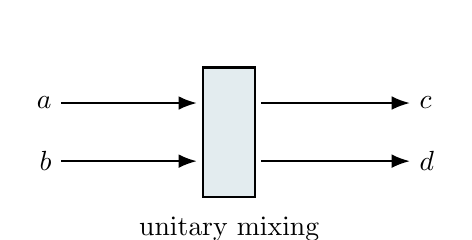
\begin{tikzpicture}[>=Latex,scale=.82]
\draw[thick,fill=accent!12] (2.5,.8) rectangle (3.3,2.8);
\draw[->,thick] (.3,2.25)--(2.4,2.25);
\draw[->,thick] (.3,1.35)--(2.4,1.35);
\draw[->,thick] (3.4,2.25)--(5.7,2.25);
\draw[->,thick] (3.4,1.35)--(5.7,1.35);
\node[left] at (.3,2.25){\(a\)};
\node[left] at (.3,1.35){\(b\)};
\node[right] at (5.7,2.25){\(c\)};
\node[right] at (5.7,1.35){\(d\)};
\node at (2.9,.3){unitary mixing};
\end{tikzpicture}
\end{center}

\subsection{Multiphoton calculations use creation operators}
When photons are input in known number states,
write the input with raising operators. For
the balanced convention
\[
a^\dagger=\frac{c^\dagger+d^\dagger}{\sqrt2},
\qquad
b^\dagger=\frac{c^\dagger-d^\dagger}{\sqrt2},
\]
the transformation of \(\ket{1,1}\) is
\[
\begin{aligned}
a^\dagger b^\dagger\ket0
&=\tfrac12(c^\dagger+d^\dagger)
(c^\dagger-d^\dagger)\ket0\\
&=\tfrac12[(c^\dagger)^2-(d^\dagger)^2]\ket0\\
&=\boxed{\frac{\ket{2,0}-\ket{0,2}}{\sqrt2}}.
\end{aligned}
\]
The absence of a \(\ket{1,1}\) term means
zero probability of detecting one photon
in each output. This is Hong--Ou--Mandel
(HOM) interference.

\subsection{Where the HOM cancellation comes from}
Two indistinguishable possibilities lead to
a coincidence: both photons transmit, or
both reflect. Their probability \emph{amplitudes}
have opposite signs and cancel at a balanced splitter.
If the photons have distinguishable wavepackets,
those alternatives no longer interfere completely.
For ideal overlap parameter \(\eta\in[0,1]\),
defined as the squared temporal/spectral-mode overlap,
\[
P(\text{coincidence})=\frac{1-\eta}{2}.
\]
At \(\eta=0\), the classical independent-path
coincidence probability is \(1/2\). At \(\eta=1\),
HOM bunching gives zero.

\begin{worked}{Two photons enter the same port}
For \(\ket{2,0}=(a^\dagger)^2\ket0/\sqrt2\),
\[
\ket{2,0}\longrightarrow
\tfrac12\ket{2,0}+\tfrac1{\sqrt2}\ket{1,1}
+\tfrac12\ket{0,2}.
\]
The output probabilities are \(1/4,1/2,1/4\).
For \(\ket{1,1}\) input, by contrast, the
coincidence probability is \emph{zero}.
Different input states lead to different
interference and photon-counting patterns.
\end{worked}

\subsection{Arbitrary \(n\) photons and coherent input}
A fixed \(n\)-photon input gives the binomial result
\[
\ket{n,0}\mapsto
\sum_{k=0}^n\sqrt{\binom nk}\,t^kr^{n-k}\ket{k,n-k}.
\]
A coherent input \(\ket\alpha_a\ket0_b\)
instead produces a \emph{product} of coherent
outputs \(\ket{t\alpha}_c\ket{r\alpha}_d\)
(up to phases). This follows by substituting
the creation-operator transformation into
the exponential Fock expansion.

\subsection{What a detector measures}
An ideal number-resolving detector distinguishes
\(n=0,1,2,\ldots\). A threshold detector
only reports vacuum or at least one photon.
For \(n\) incident photons and single-photon
detection efficiency \(\eta_d\), the probability
of \emph{no click} is
\[
P(0\ \text{clicks}\mid n)=(1-\eta_d)^n,
\]
neglecting dark counts. Real detection
requires careful treatment of loss, dark counts
and finite time resolution.

\subsection{Homodyne detection accesses field quadratures}
Interfere a weak signal \(a\) with a strong coherent
local oscillator \(\beta=|\beta|e^{i\theta}\).
Subtract the output photodetector currents.
The dominant difference term is proportional to
\[
\beta^*a+\beta a^\dagger
=|\beta|[ae^{-i\theta}+a^\dagger e^{i\theta}].
\]
A local-oscillator phase change selects
a different quadrature rather than a different
photon-number observable.

\begin{checkpoint}
For optical circuits: define input modes,
choose a phase convention, transform operators,
restore the \(\sqrt{n!}\) factors, add
amplitudes, and only then square them.
\end{checkpoint}

\unit{Quadratures and phase-space pictures}
\unitref{W1L3 and W3L1; homodyne lectures}
\subsection{What are the two quadratures of a wave?}
A monochromatic classical electric field can be written
\[
E(t)=A\cos\omega t+B\sin\omega t.
\]
The coefficients \(A,B\) specify its amplitude and
phase. They are not frequency and amplitude: the
\emph{frequency} \(\omega\) is already fixed by
the mode. Quantum mechanically, define
\[
\boxed{x=a+a^\dagger,\qquad
p=i(a^\dagger-a),\qquad a=(x+ip)/2.}
\]
The commutator is
\[
[x,p]=[a+a^\dagger,i(a^\dagger-a)]
=2i.
\]
Heisenberg's inequality gives
\[
\boxed{\Delta x\,\Delta p\ge1.}
\]
In this course convention the vacuum has
\((\Delta x)^2=(\Delta p)^2=1\).
A textbook using \(x=(a+a^\dagger)/\sqrt2\)
has vacuum variance \(1/2\); no physics
changes, only the scaling.

\subsection{The meaning of the phase-space plane}
For a coherent state \(\ket\alpha\),
\[
\langle x\rangle=2\operatorname{Re}\alpha,\quad
\langle p\rangle=2\operatorname{Im}\alpha,\quad
(\Delta x)^2=(\Delta p)^2=1.
\]
Thus a coherent state looks like a
vacuum uncertainty circle displaced from the
origin. Its centre identifies a classical-like
field amplitude; its width encodes unavoidable
quantum fluctuations.

\begin{center}
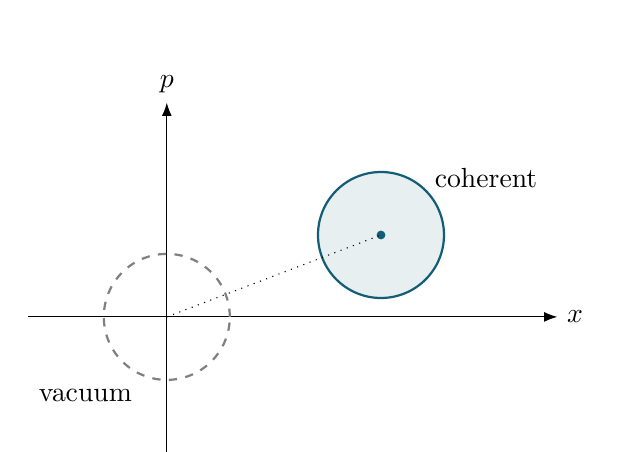
\begin{tikzpicture}[>=Latex,scale=.8]
\draw[->](-2.2,0)--(6.2,0)node[right]{\(x\)};
\draw[->](0,-2.3)--(0,3.4)node[above]{\(p\)};
\draw[gray,dashed,thick](0,0)circle(1);
\draw[accent,fill=accent!10,thick](3.4,1.3)circle(1);
\fill[accent](3.4,1.3)circle(.07);
\draw[dotted](0,0)--(3.4,1.3);
\node[below left]at(-.4,-1){vacuum};
\node[above right]at(4.1,1.9){coherent};
\end{tikzpicture}
\end{center}

\subsection{Rotated quadratures}
For a local-oscillator phase \(\theta\),
\[
\boxed{X_\theta=ae^{-i\theta}
+a^\dagger e^{i\theta}
=x\cos\theta+p\sin\theta.}
\]
Homodyne detection measures the probability
distribution of \(X_\theta\). At \(\theta=0\)
it measures \(x\); at \(\theta=\pi/2\)
it measures \(p\). Measuring distributions
over many angles enables optical homodyne
tomography. The phase-space distribution
is reconstructed from different projections,
rather than measured pointwise with
arbitrarily sharp \(x,p\) simultaneously.

\begin{worked}{Rotate the local oscillator}
Take \(\alpha=1+i\). Then
\(\langle x\rangle=\langle p\rangle=2\).
At \(\theta=\pi/4\),
\[
\langle X_{\pi/4}\rangle
=2\cos(\pi/4)+2\sin(\pi/4)=2\sqrt2.
\]
Its variance remains 1, since coherent
vacuum noise is equally distributed
in all directions.
\end{worked}

\subsection{Three complementary quasiprobabilities}
The Wigner function \(W(x,p)\) represents
a quantum state in phase space. Its
marginals give measurable quadrature
probabilities, but some quantum states
have negative Wigner regions.
The Husimi function is
\[
Q(\alpha)=\frac1\pi\bra\alpha\rho\ket\alpha,
\]
which is always nonnegative and is smoother
than the Wigner function. The
Glauber--Sudarshan representation is
\[
\rho=\int P(\alpha)\ket\alpha\bra\alpha\,d^2\alpha.
\]
Here \(P\) can be singular or nonpositive:
it is \emph{not always} a classical
probability distribution.
All three describe the same \(\rho\), but
highlight different physical properties.

\subsection{Gaussian states and covariance}
For \(R=(x,p)^T\), define
\[
d_i=\langle R_i\rangle,\qquad
V_{ij}=\tfrac12\langle\Delta R_i\Delta R_j+
\Delta R_j\Delta R_i\rangle.
\]
A Gaussian state is completely specified
by \(d,V\). Coherent and squeezed Gaussian
states have Gaussian Wigner functions.
A lossless linear transformation \(R'=SR\)
acts as \(d'=Sd,\ V'=SVS^T\).
An open-system Gaussian channel generally adds
noise: \(V'=SVS^T+N\).

\begin{checkpoint}
Phase space is useful for \emph{states of modes}.
Quadrature \(x\) is not position of a photon
and \(p\) is not its momentum. They are
conjugate field-amplitude variables.
\end{checkpoint}

\unit{Squeezing, coherence and photon correlations}
\unitref{W3L2, W3L3; W6L3; Assignment 1}
\subsection{What is actually being squeezed?}
Squeezing changes \emph{field quadrature
uncertainties}. A vacuum state has equal
variance 1 in \(x,p\) with our convention.
For real \(r\), a squeezing operator can be defined as
\[
S(r)=\exp\left[\frac r2(a^2-a^{\dagger2})\right].
\]
Its Bogoliubov action is
\[
S^\dagger aS=a\cosh r-a^\dagger\sinh r.
\]
Consequently
\[
S^\dagger xS=e^{-r}x,\qquad
S^\dagger pS=e^{r}p,
\]
and the squeezed vacuum \(S(r)\ket0\) has
\[
\boxed{(\Delta x)^2=e^{-2r},\quad
(\Delta p)^2=e^{2r},\quad
\Delta x\,\Delta p=1.}
\]
The uncertainty ellipse becomes narrow in
one direction and wide in the other;
the product does \emph{not} violate Heisenberg.

\begin{center}
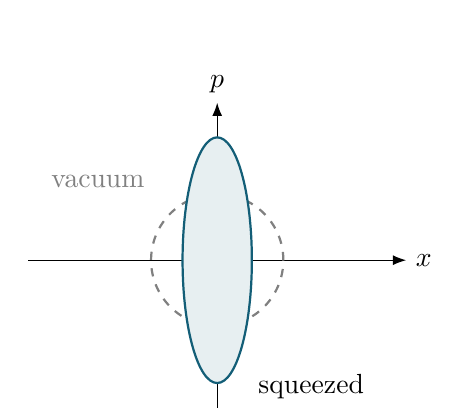
\begin{tikzpicture}[>=Latex,scale=.8]
\draw[->](-3,0)--(3,0)node[right]{\(x\)};
\draw[->](0,-2.5)--(0,2.5)node[above]{\(p\)};
\draw[dashed,gray,thick](0,0)circle(1.05);
\draw[accent,thick,fill=accent!10](0,0)ellipse(.55 and 1.95);
\node[below right]at(.5,-1.65){squeezed};
\node[above left,gray]at(-1,1){vacuum};
\end{tikzpicture}
\end{center}

\subsection{How can vacuum contain squeezed photons?}
The squeezed vacuum has
\(\langle a\rangle=0\), but its mean
photon number is
\[
\boxed{\langle n\rangle=\sinh^2r.}
\]
It contains even-number superposition components
produced by a parametric process.
A \emph{displaced squeezed} state has nonzero
mean field as well as anisotropic noise.
The order of \(D(\alpha)\) and \(S(r)\)
matters if a calculation asks for the
total number population, because
the two operators do not generally commute.

\subsection{Squeezing helps only the measured direction}
If a signal shifts the \(x\)-mean by
\(\delta x\), the noise-limited sensitivity
scales as \(\delta x/\Delta x\).
An \(x\)-squeezed probe reduces
\(\Delta x\) by \(e^{-r}\) and improves this
signal-to-noise ratio. But if one measures
the \(p\) quadrature instead, the noise
is \emph{larger}. The optical phase of
the local oscillator must therefore
match the squeezing axis.

\begin{worked}{How loss spoils squeezing}
Take input \(x\)-quadrature variance
\(V_{\rm in}=e^{-2r}=1/4\), and a channel
with power transmission \(\eta=0.8\).
A vacuum environment enters through the
unobserved beam-splitter port:
\[
V_{\rm out}=\eta V_{\rm in}+(1-\eta)V_{\rm vac}
=0.8(1/4)+0.2(1)=\boxed{0.40}.
\]
The output is still squeezed relative
to vacuum (\(V_{\rm out}<1\)), but
not as strongly as the input.
\end{worked}

\subsection{What does coherence measure?}
First-order coherence measures field
correlations across space or time:
\[
G^{(1)}(t,t+\tau)
=\langle a^\dagger(t)a(t+\tau)\rangle.
\]
It is related to ordinary interference
visibility and spectral linewidth.
Second-order coherence measures correlated
photon arrivals,
\[
G^{(2)}(t,t+\tau)=
\langle a^\dagger(t)a^\dagger(t+\tau)
a(t+\tau)a(t)\rangle.
\]
Normalised \(g^{(2)}(0)>1\) describes
bunching; \(g^{(2)}(0)<1\) describes
antibunching, which is nonclassical
for a stationary single-mode field
under conventional assumptions.
An experiment can reveal coherence
without being a direct measurement
of a particular optical phase.

\subsection{Pair production and heralding}
A two-mode squeezed vacuum
\(\sum_n\lambda^n\ket{n,n}\)
contains signal--idler number correlations.
If the idler is unobserved,
the signal looks thermal. If a detector
heralds exactly one idler photon,
the conditional signal is \(\ket1\).
This is possible because measurement
changes the state of the \emph{remaining}
subsystem, even if the global evolution
before detection was unitary.

\begin{checkpoint}
Squeezing concerns quadrature noise.
Bunching concerns photon arrival statistics.
First-order coherence concerns field
correlations. These are related but
not interchangeable ideas.
\end{checkpoint}

\partmarking{II}{Applications of optics}
\unit{Photonic qubits and the Bloch sphere}
\unitref{W4L1 and W4L2; Assignment 2}
\subsection{From an optical mode to a qubit}
A qubit is a normalised superposition of two
basis states, \(\ket\psi=\alpha\ket0+\beta\ket1\)
with \(|\alpha|^2+|\beta|^2=1\).
For photons there are several useful
physical encodings:
\[
\begin{array}{l|cc}
&\ket{0_L}&\ket{1_L}\\\hline
\text{polarisation}&\ket H&\ket V\\
\text{dual rail (path)}&\ket{1,0}&\ket{0,1}\\
\text{time bin}&\ket{\rm early}&\ket{\rm late}
\end{array}
\]
In dual rail, one photon is present across
the two logical modes. The state \(\ket{0,0}\)
is an erasure/vacuum state outside the
logical computational subspace, not logical zero.

\subsection{What the Bloch sphere represents}
Ignoring a global phase, every \emph{pure}
single-qubit state can be parameterised as
\[
\boxed{\ket\psi=\cos(\theta/2)\ket0+
e^{i\phi}\sin(\theta/2)\ket1.}
\]
The Bloch vector is
\(\mathbf r=(\sin\theta\cos\phi,
\sin\theta\sin\phi,\cos\theta)\).
The poles represent \(\ket0,\ket1\);
the equator contains equal-amplitude
superpositions with different relative phases.
A mixed state has density matrix
\[
\rho=\tfrac12(I+\mathbf r\cdot\boldsymbol\sigma),
\quad |\mathbf r|\le1,
\]
and lies inside the sphere.

\subsection{Quantum gates are rotations}
The Pauli matrices are
\[
X=\begin{pmatrix}0&1\\1&0\end{pmatrix},\quad
Y=\begin{pmatrix}0&-i\\i&0\end{pmatrix},\quad
Z=\begin{pmatrix}1&0\\0&-1\end{pmatrix}.
\]
The Hadamard gate is
\(H=(X+Z)/\sqrt2\), with
\(H\ket0=(\ket0+\ket1)/\sqrt2\).
A rotation generated by a Pauli operator is
\[
R_j(\vartheta)=e^{-i\vartheta\sigma_j/2}
=\cos(\vartheta/2)I-
i\sin(\vartheta/2)\sigma_j.
\]
On a path qubit, a beam splitter acts as
a rotation and a relative optical phase
acts as a \(Z\)-rotation. On a
polarisation qubit, appropriately oriented
wave plates implement the same mathematics.
Physical optical hardware supplies a
\emph{representation} of the logical gate.

\begin{worked}{A relative phase is observable}
Start with \(\ket+\!=\!(\ket0+\ket1)/\sqrt2\).
A phase shifter on logical \(\ket1\)
creates \((\ket0+e^{i\phi}\ket1)/\sqrt2\).
Measuring immediately in the \(Z\) basis
gives \(1/2,1/2\), regardless of \(\phi\).
But applying a Hadamard before measurement gives
\[
P(0)=\left|\frac{1+e^{i\phi}}2\right|^2
=\boxed{\cos^2(\phi/2)}.
\]
The interferometer converts a relative
phase into a measurable number probability.
\end{worked}

\subsection{Entanglement is not classical correlation}
Consider
\[
\ket{\Phi^+}=\frac{\ket{00}+\ket{11}}{\sqrt2}.
\]
It is a pure \emph{joint} state that cannot
be factored into independent states
of Alice and Bob. Trace out Bob:
\[
\rho_A=\operatorname{Tr}_B
\ket{\Phi^+}\bra{\Phi^+}=\tfrac12I.
\]
Alice's measurement is locally random,
yet her result matches Bob's if both
measure in the same \(Z\) basis.
In the \(X\) basis,
\(\ket{\Phi^+}=(\ket{++}+\ket{--})/\sqrt2\),
so the correlations persist there too.

\subsection{Partial trace is a practical calculation}
For a two-qubit density operator expressed
as \(\rho=\sum_{ijkl}\rho_{ij,kl}\ket{i,j}\bra{k,l}\),
\[
\boxed{\operatorname{Tr}_B\rho=
\sum_{i,k,j}\rho_{ij,kj}\ket i\bra k.}
\]
The two indices of the discarded subsystem
must agree. This erases correlations not
accessible to measurements on \(A\) alone.

\begin{checkpoint}
A pure entangled pair can have \emph{mixed}
single-photon reduced states. The Bloch sphere
describes a qubit's local state; it does not
by itself encode all joint correlations.
\end{checkpoint}

\unit{Quantum communication: teleportation, dense coding and QKD}
\unitref{W4L2--W4L3; Assignment 2; 2025 Q4(e)}
\subsection{Three communication tasks: do not confuse them}
Teleportation transfers an \emph{unknown qubit state}
using a shared entangled pair and two classical bits.
Dense coding sends \emph{two classical bits} using
one transmitted qubit and one pre-shared Bell pair.
Quantum key distribution (QKD) establishes shared
secret classical bits and tests whether an
eavesdropper could have learned them.
The resource accounting is different in each task.

\subsection{Teleportation as a calculation}
Suppose Alice holds \(\ket\psi=\alpha\ket0+\beta\ket1\).
Alice and Bob also share
\(\ket{\Phi^+}_{AB}=(\ket{00}+\ket{11})/\sqrt2\).
Alice performs CNOT from the unknown qubit
onto her half of the Bell pair, then a Hadamard
on the unknown qubit. Rewriting in Alice's
two-qubit computational basis gives
\[
\begin{aligned}
&\ket\psi\ket{\Phi^+}_{AB}\longrightarrow\\
&\quad \frac12[
\ket{00}_A\ket\psi_B+
\ket{01}_A X\ket\psi_B+
\ket{10}_A Z\ket\psi_B+
\ket{11}_A XZ\ket\psi_B],
\end{aligned}
\]
up to a harmless convention-dependent phase
on the last branch. Alice measures her
two qubits and sends the result (two bits).
Bob applies the appropriate Pauli correction:
\[
00\to I,\qquad01\to X,\qquad10\to Z,
\qquad11\to ZX
\]
(with the order consistent with the state branch).
The outcome is always Bob's \(\ket\psi\).
The original input has been consumed, so
this does not clone the state. Bob cannot
recover \(\ket\psi\) before Alice's classical
message arrives.

\subsection{Dense coding uses four Bell messages}
Starting from \(\ket{\Phi^+}\), Alice can apply
\[
I\to\Phi^+,\quad X\to\Psi^+,\quad
Z\to\Phi^-,\quad XZ\to\Psi^-
\]
(up to global phase).
Bob would ideally discriminate all four
orthogonal Bell states after receiving Alice's
photon. The standard passive beam-splitter
and number-detection analyser distinguishes
\(\Psi^\pm\) through their port/polarisation
patterns, but not \(\Phi^+\) from \(\Phi^-\).
Thus the ordinary no-ancilla linear-optical
Bell measurement is not deterministic;
its unambiguous success probability for
equiprobable Bell states is \(1/2\).

\subsection{BB84: prepare, measure, sift, test}
BB84 uses two conjugate bases,
\[
Z:\{\ket H,\ket V\},\qquad
X:\{\ket D,\ket A\},\quad
\ket{D/A}=\frac{\ket H\pm\ket V}{\sqrt2}.
\]
Alice randomly chooses a basis and bit;
Bob randomly chooses a measurement basis.
After transmission they announce \emph{bases},
not retained secret bit values, and keep
measurements where their bases matched.
Independent uniform bases match with probability
\(\boxed{1/2}\).
With channel and detector efficiencies
\(\eta_{\rm ch},\eta_d\), the expected sifted
number out of \(N\) ideal single-photon pulses is
\[
\boxed{\mathbb E[N_{\rm sift}]
=\frac N2\eta_{\rm ch}\eta_d},
\]
before testing, reconciliation and privacy
amplification.

\begin{worked}{Why intercept--resend creates 25\% errors}
Condition on a sifted event: Bob used Alice's basis.
An intercept--resend Eve chooses that basis
with probability \(1/2\), making no error.
If Eve used the wrong basis (probability \(1/2\)),
Bob's subsequently recovered bit is wrong with
probability \(1/2\). Therefore
\[
\boxed{\mathrm{QBER}=\tfrac12(0)+
\tfrac12(\tfrac12)=\tfrac14.}
\]
If \(m=20\) independent sifted test bits are
revealed, the probability of noticing at
least one error in this simple model is
\(1-(3/4)^{20}\approx0.9968\).
These public test bits are discarded.
\end{worked}

\subsection{What makes a practical key secure?}
Alice and Bob estimate a quantum bit error rate,
perform error correction and then privacy
amplification. Revealed parity information
and imperfect sources affect the final key rate.
Security requires an \emph{authenticated}
classical discussion channel as well as quantum
transmission. Multi-photon weak-laser pulses
are not identical to ideal single-photon states;
decoy-state methods are one way to address
source imperfections in implementations.

\begin{checkpoint}
Teleportation is not instantaneous transport
of an object. Dense coding needs prior
entanglement. BB84 detects disturbance
through \emph{incompatible measurements},
not through a secret choice of quantum bases.
\end{checkpoint}

\unit{Noise, loss and quantum channels}
\unitref{W5L1; Week 5 tutorial}
\subsection{Why a subsystem does not evolve unitarily}
For an isolated quantum system,
\(\rho'=U\rho U^\dagger\).
An optical mode in the laboratory interacts
with unobserved environmental degrees of
freedom: lost photons, thermally excited
modes, unwanted phase fluctuations and detectors.
If the environment starts in \(\rho_E\),
\[
\boxed{\rho'_S=
\operatorname{Tr}_E[
U_{SE}(\rho_S\otimes\rho_E)U_{SE}^\dagger].}
\]
The joint evolution is unitary but the reduced
system evolution generally is not. Tracing out
the environment is an \emph{average over
unobserved information}, not a measurement
that selects a particular outcome.

\subsection{Loss as a beam splitter with vacuum}
Introduce an initially empty environment mode \(e\):
\[
a_{\rm out}=\sqrt\eta\,a_{\rm in}
+\sqrt{1-\eta}\,e_{\rm in}.
\]
This is the physically correct quantum loss
model; replacing \(a\) by \(\sqrt\eta a\)
alone would give
\([a_{\rm out},a_{\rm out}^\dagger]=\eta\ne1\).
The environment operator supplies the vacuum
noise that preserves the commutator.
For a single photon,
\[
\ket{1,0}_{S,E}\longrightarrow
\sqrt\eta\ket{1,0}
+\sqrt{1-\eta}\ket{0,1}.
\]
Tracing over the environment gives
\[
\boxed{\rho'_S=\eta\ket1\bra1+
(1-\eta)\ket0\bra0.}
\]
The probability of having a photon is \(\eta\);
the environment is responsible for the mixture.

\subsection{Kraus operators: a system-only description}
The same channel can be written
\[
\boxed{\mathcal E(\rho)=\sum_kK_k\rho K_k^\dagger,
\quad\sum_kK_k^\dagger K_k=I.}
\]
For a single-rail state supported on
\(\{\ket0,\ket1\}\), loss has
\[
K_0=\begin{pmatrix}1&0\\0&\sqrt\eta\end{pmatrix},
\qquad
K_1=\begin{pmatrix}0&\sqrt{1-\eta}\\0&0\end{pmatrix}.
\]
The \(K_0\) branch contains no environment
excitation, while \(K_1\) represents losing
the photon. These are \emph{not} two
alternative deterministic maps; they form
one trace-preserving channel when summed.

\begin{worked}{A superposition passes through loss}
For \(\ket\psi=\alpha\ket0+\beta\ket1\),
\[
\rho'=\sum_kK_k\ket\psi\bra\psi K_k^\dagger
=\boxed{\begin{pmatrix}
|\alpha|^2+(1-\eta)|\beta|^2&
\sqrt\eta\,\alpha\beta^*\\
\sqrt\eta\,\alpha^*\beta&
\eta|\beta|^2
\end{pmatrix}}.
\]
Check the trace: it is 1.
The excited population is suppressed by
\(\eta\), but vacuum--one-photon
coherence by \(\sqrt\eta\).
For \(\eta=1\) the original pure state is
recovered. For \(\eta=0\) the output is vacuum.
\end{worked}

\subsection{Phase damping is different from photon loss}
Phase noise can suppress coherences without
changing photon-number probabilities.
For a number basis, a random phase
\(e^{i\phi\hat n}\) has no effect on
diagonal populations but averages away
off-diagonal terms such as \(\ket0\bra1\).
A simple dephasing channel acts on a qubit as
\[
\rho_{01}\mapsto\lambda\rho_{01},\quad
\rho_{00}\mapsto\rho_{00},\quad
\rho_{11}\mapsto\rho_{11},
\qquad0\le\lambda\le1.
\]
Hence direct photon counting can miss phase
noise that is obvious in homodyne detection.

\subsection{When measurement becomes conditioning}
If an environmental or ancilla outcome \(k\)
is actually observed and kept, use
\[
\tilde\rho_k=K_k\rho K_k^\dagger,\quad
p_k=\operatorname{Tr}\tilde\rho_k,\quad
\boxed{\rho_k=\tilde\rho_k/p_k}.
\]
This is a trace-decreasing \emph{conditional}
operation. Summing over all outcomes instead
recovers the unconditional channel.
For conditional photon subtraction, a weak
beam splitter followed by a one-photon
detector click implements an operator
approximately proportional to \(a\).
It weights higher Fock components by \(\sqrt n\),
not simply removing one photon deterministically.

\begin{checkpoint}
Ask which information is available.
If the environment is ignored, trace it
out or sum Kraus branches. If a detector
outcome is heralded, \emph{select and
renormalise} that branch, retaining its
separate success probability.
\end{checkpoint}

\unit{Damping, Langevin noise and master equations}
\unitref{W5L2; 2024 Q4; 2025 Q4}
\subsection{Two ways of describing the same physics}
The Heisenberg picture evolves operators;
the Schr\"odinger picture evolves density matrices.
For a closed system,
\[
\dot O=\frac{i}{\hbar}[H,O],\qquad
\dot\rho=-\frac{i}{\hbar}[H,\rho].
\]
An open system also has damping and fluctuations,
because it couples to many unobserved bath modes.
The Markov approximation replaces bath memory
by effectively instantaneous noise; it is
useful when bath correlations decay quickly
compared with the system dynamics.

\subsection{Where the quantum Langevin equation comes from}
A cavity mode \(a\) coupled weakly to
a continuum of oscillators \(b_\omega\)
has a Hamiltonian of the schematic form
\[
H/\hbar=\omega_ca^\dagger a+
\int\omega b_\omega^\dagger b_\omega d\omega+
i\int\kappa(\omega)
(a^\dagger b_\omega-b_\omega^\dagger a)d\omega.
\]
One first solves the bath equation for \(b_\omega(t)\);
substituting it back into the cavity equation
produces a \emph{damping} term and an
\emph{input noise} term. In a frame rotating
at the cavity resonance,
\[
\boxed{\dot a=-\frac\gamma2a+
\sqrt\gamma\,a_{\rm in}(t)}
\]
for an undriven cavity with one damping port.
The noise operator is not an optional
classical disturbance: it ensures that
operator commutators remain physically valid.

\subsection{Fourier solving is usually easiest}
Define
\(\tilde a(\omega)=\int_{-\infty}^\infty
a(t)e^{-i\omega t}\,dt\), so
\(\widetilde{\dot a}=i\omega\tilde a\)
when boundary terms vanish.
Then
\[
(i\omega+\gamma/2)\tilde a
=\sqrt\gamma\,\tilde a_{\rm in},
\qquad
\boxed{\tilde a=
\frac{\sqrt\gamma}{\gamma/2+i\omega}
\tilde a_{\rm in}}.
\]
The denominator is the cavity susceptibility.
Near zero detuning it has a large response;
far from resonance the response is smaller.
A consistent Fourier convention is essential
because another sign convention replaces
\(i\omega\) by \(-i\omega\).

\subsection{Input--output theory}
With one common convention,
\[
a_{\rm out}=\sqrt\gamma\,a-a_{\rm in}.
\]
Eliminating the intracavity operator gives
a frequency-dependent relation between
input and output fields. For a two-port
cavity with \(\gamma=\gamma_1+\gamma_2\),
\[
\dot a=-\frac\gamma2a+
\sqrt{\gamma_1}a_{{\rm in},1}
+\sqrt{\gamma_2}a_{{\rm in},2},
\]
\[
\boxed{
\tilde a_{{\rm out},1}
=\frac{\gamma_1-\gamma/2-i\omega}
{\gamma/2+i\omega}\tilde a_{{\rm in},1}
+\frac{\sqrt{\gamma_1\gamma_2}}
{\gamma/2+i\omega}\tilde a_{{\rm in},2}.}
\]
At \(\omega=0\) and \(\gamma_1=\gamma_2\)
the coherent reflection coefficient vanishes.
But the second input's vacuum fluctuations
must remain in the \emph{field operator}.

\subsection{The Lindblad master equation}
After tracing over a Markovian bath, a general
trace-preserving reduced evolution is
\[
\boxed{\dot\rho=-\frac{i}{\hbar}[H,\rho]+
\sum_j\gamma_j\mathcal D[L_j]\rho},
\]
where
\[
\mathcal D[L]\rho=L\rho L^\dagger
-\frac12(L^\dagger L\rho+\rho L^\dagger L).
\]
A cavity losing photons into vacuum has
\(L=a\), while a two-level atom decaying
spontaneously has \(L=\sigma_-\).
Pure dephasing can be modelled with a
Hermitian jump operator related to \(\sigma_z\).
The jump operator tells you \emph{which
physical transition the environment causes}.

\begin{worked}{Photon number decays exponentially}
For zero-temperature cavity loss,
\(\dot\rho=\gamma\mathcal D[a]\rho\).
Use \(\frac{d}{dt}\langle n\rangle
=\operatorname{Tr}(n\dot\rho)\) and
\([n,a]=-a\). After rearrangement,
\[
\frac{d}{dt}\langle n\rangle
=-\gamma\langle n\rangle.
\]
Hence
\[
\boxed{\langle n(t)\rangle
=\langle n(0)\rangle e^{-\gamma t}}.
\]
The field amplitude decays at half
that exponent (\(\gamma/2\)), explaining
the factor 2 in the Langevin equation.
\end{worked}

\subsection{Parametric squeezing in a cavity}
For interaction
\(H_I=(i\hbar\chi/2)(a^2-a^{\dagger2})\),
the Heisenberg commutator contributes
\(-\chi a^\dagger\) to \(\dot a\).
Define \(X_+=a+a^\dagger\), giving
\[
\dot X_+=-(\gamma/2+\chi)X_+
+\sqrt\gamma X_{+,\rm in}.
\]
The output noise transfer factor leads to
\[
\boxed{V_+(\omega)=
\frac{(\gamma/2-\chi)^2+\omega^2}
{(\gamma/2+\chi)^2+\omega^2}}
\]
for unit vacuum input spectrum and
\(0<\chi<\gamma/2\).
The \emph{variance} comes from
field-fluctuation correlations, not
the square of the mean field.

\begin{checkpoint}
For a Langevin exam question:
identify the Hamiltonian and port rates,
calculate the commutator, Fourier transform,
apply the exact input--output sign
convention, then evaluate the noise spectrum.
\end{checkpoint}

\unit{Conditional optics: how measurement becomes a gate}
\unitref{W5L3; Week 6 tutorial; Assignment 2}
\subsection{A surprising capability of linear optics}
Beam splitters and phase shifters implement
linear unitary transformations of optical
modes. They cannot directly create a
deterministic interaction between two
photons. But combining these optical
elements with ancilla photons and
\emph{postselected} photodetection can
implement an effective nonlinear operation
on a conditional subensemble.
The cost is that some runs must be rejected.

\subsection{One outcome, one Kraus operator}
If the joint state of signal and ancilla
is \(U(\ket\psi\otimes\ket{\rm anc})\)
and the ancilla detector yields \(k\),
the signal's unnormalised output is
\[
\ket{\tilde\psi_k}
={}_{\rm anc}\bra k U
(\ket\psi\otimes\ket{\rm anc}),
\]
or \(\tilde\rho_k=K_k\rho K_k^\dagger\).
The probability of this outcome is
\(p_k=\operatorname{Tr}\tilde\rho_k\);
\(\rho_k=\tilde\rho_k/p_k\) is the
normalised state for successful trials.
Do \emph{not} normalise before calculating
the success probability.

\subsection{Photon subtraction}
Consider a signal
\(\ket\psi=\sum_n c_n\ket n\)
mixed with vacuum at a weakly reflecting
beam splitter of transmissivity \(\eta\).
Conditioning on one photon in the
reflected output produces
\[
\boxed{K_{\rm click}\ket n\propto
\sqrt n\,\sqrt{1-\eta}\,
\eta^{(n-1)/2}\ket{n-1}.}
\]
The factor \(\sqrt n\) is the
annihilation-operator matrix element.
The factor \(\eta^{(n-1)/2}\) accounts for
the photons retained in the signal.
For \(\eta\) near 1, the operation
approximates \(a\ket\psi\), up to
an overall success amplitude.
It \emph{does not} remove a photon
deterministically from every trial.

\begin{worked}{Distinguishing nonorthogonal states probabilistically}
Take the two input states
\[
\ket{\psi_\pm}=\frac{2\ket0\pm\ket1}{\sqrt5},
\qquad \langle\psi_+|\psi_-\rangle=3/5.
\]
They cannot be perfectly distinguished by
a deterministic measurement. Use a
successful filter
\[
K_s=\tfrac12\ket0\bra0+\ket1\bra1.
\]
The unnormalised output is
\((\ket0\pm\ket1)/\sqrt5\)
with probability \(p_s=2/5\).
After normalising,
\[
\boxed{\ket{\phi_\pm}=
\frac{\ket0\pm\ket1}{\sqrt2}}.
\]
These are \emph{orthogonal}, so a
Hadamard-basis measurement now identifies
the sign, conditional on success.
The failure probability is \(3/5\);
the identical failure output contains
no information about the sign. Probabilistic
filtering does not violate no-cloning
or deterministic distinguishability.
\end{worked}

\subsection{Heralding and gate resources}
Conditional sign gates can transform selected
Fock coefficients with relative phases,
for example \(\alpha\ket0+\beta\ket1+
\gamma\ket2\) into
\(\alpha\ket0+\beta\ket1-\gamma\ket2\)
in a successful ancilla detection branch.
Such number-dependent relative phases
are effectively nonlinear operations,
even though the optical elements
before measurement were linear.
This idea is used in measurement-induced
photonic computation, with ancilla states,
feed-forward and suitable encoding.

\subsection{Entanglement distillation}
Two noisy Bell pairs can be processed
with bilateral gates and local measurements
to keep one pair only when parity checks
succeed. For the simple ensemble
\[
\rho=p\ket{\Phi^+}\bra{\Phi^+}
+(1-p)\ket{\Psi^+}\bra{\Psi^+},
\]
a recurrence protocol keeps matching
error labels with
\[
p_{\rm success}=p^2+(1-p)^2,
\quad
\boxed{p'=\frac{p^2}{p^2+(1-p)^2}}.
\]
For \(p=0.8\), the retained fidelity
rises to \(p'\approx0.9412\),
but the pair is obtained with probability
\(0.68\) from two initial pairs.
Entanglement quality improves at the
expense of throughput.

\begin{checkpoint}
Always report \emph{both} the conditional
output state and its success probability.
Distinguish a trace-preserving quantum
channel from a selected, trace-decreasing
instrument outcome.
\end{checkpoint}

\unit{One atom, one photon: Jaynes--Cummings physics}
\unitref{W6L1; W6L2; Week 6 tutorial}
\subsection{Why a two-level atom is a useful model}
An atom has many levels, but when a narrow-band
cavity is tuned close to a single transition
\(\ket g\leftrightarrow\ket e\), the other
levels may be neglected to a good approximation.
The atom then behaves like a spin-\(1/2\)
system with
\[
\sigma_+=\ket e\bra g,\quad
\sigma_-=\ket g\bra e,\quad
\sigma_z=\ket e\bra e-\ket g\bra g.
\]
One photon of frequency \(\omega_c\) has
the right energy to excite the atom if
\(\omega_c\approx\omega_a\).
The dipole interaction
\(H_{\rm int}=-\mathbf d\cdot\mathbf E\)
contains products of photon and atomic
raising/lowering operators.

\subsection{Rotating-wave approximation}
Terms \(a\sigma_+\) and \(a^\dagger\sigma_-\)
exchange excitation between atom and field.
The counter-rotating combinations
\(a\sigma_-\) and \(a^\dagger\sigma_+\)
change excitation number by two and
oscillate rapidly near resonance.
If \(g\ll\omega_a,\omega_c\), the
rotating-wave approximation retains
the slowly varying terms:
\[
\boxed{H_{\rm JC}=
\hbar\omega_c a^\dagger a+
\hbar\omega_a\sigma_+\sigma_-+
\hbar g(a\sigma_++a^\dagger\sigma_-).}
\]
The excitation operator
\(N=a^\dagger a+\sigma_+\sigma_-\)
commutes with \(H_{\rm JC}\):
excitations move, but their total number is conserved.

\subsection{Reduce the problem to a two-state block}
For a fixed total excitation,
the coupled states are
\(\ket{e,n}\) and \(\ket{g,n+1}\).
After subtracting a common energy, the
Hamiltonian block is
\[
\frac{H_n}{\hbar}=
\frac12\begin{pmatrix}
\Delta&2g\sqrt{n+1}\\
2g\sqrt{n+1}&-\Delta
\end{pmatrix},
\quad \Delta=\omega_a-\omega_c.
\]
Its eigenfrequency separation is
\[
\boxed{\Omega_n=
\sqrt{\Delta^2+4g^2(n+1)}}.
\]
The factor \(\sqrt{n+1}\) comes from
\(a^\dagger\ket n=\sqrt{n+1}\ket{n+1}\).
It is a directly observable signature
of a quantised cavity field.

\begin{worked}{Vacuum Rabi oscillation}
Begin in \(\ket{e,0}\) at resonance
(\(\Delta=0\)). The interaction block is
\(\hbar g\sigma_x\), so
\[
\ket{\psi(t)}
=\cos(gt)\ket{e,0}
-i\sin(gt)\ket{g,1}.
\]
Thus
\[
\boxed{P_e(t)=\cos^2(gt),\quad
P_{g,1}(t)=\sin^2(gt)}.
\]
At \(t=\pi/(2g)\) the atom has emitted
one photon into the cavity.
At a full period \(t=\pi/g\),
the excitation has returned to the atom.
\end{worked}

\subsection{From one atom to many: Tavis--Cummings}
For \(N\) identical emitters with the same
coupling phase,
\[
H_I=\hbar g(aJ_++a^\dagger J_-),\quad
J_\pm=\sum_{i=1}^N\sigma_\pm^{(i)}.
\]
For two atoms with one excitation, define
\[
\ket S=\frac{\ket{eg}+\ket{ge}}{\sqrt2},
\quad
\ket A=\frac{\ket{eg}-\ket{ge}}{\sqrt2}.
\]
Because
\[
J_-\ket S=\sqrt2\ket{gg},\qquad
J_-\ket A=0,
\]
the symmetric state is \emph{bright},
with coupling \(\sqrt2g\);
the antisymmetric state is \emph{dark}
to the common cavity mode.

\subsection{Dicke states and superradiant enhancement}
For \(N\) symmetric spins, collective
angular-momentum labels \(J=N/2,m\)
describe a Dicke ladder. The lowering operator
has matrix element
\[
J_-\ket{J,m}=
\sqrt{(J+m)(J-m+1)}\ket{J,m-1}.
\]
If all atoms couple to a \emph{common}
radiation reservoir under appropriate
conditions, these factors enhance
collective spontaneous emission rates.
The coherent cavity-exchange enhancement
\(\sqrt N\,g\) and cooperative radiative
superradiance are related but not
identical phenomena: the reservoir and
initial state also matter.

\begin{worked}{Two-atom conservation check}
Start with \(\ket{eg,0}\).
It equals \((\ket{S,0}+\ket{A,0})/\sqrt2\).
The bright half oscillates with
\(\sqrt2g\), while the dark half stays.
Writing \(\vartheta=\sqrt2gt\),
\[
\ket{\psi(t)}
=\frac{\cos\vartheta\ket{S,0}+\ket{A,0}
-i\sin\vartheta\ket{gg,1}}{\sqrt2}.
\]
The mean cavity photon number is
\(\langle n\rangle=\tfrac12\sin^2\vartheta\).
The missing probability remains as atomic
excitation, preserving \(\langle N\rangle=1\).
\end{worked}

\begin{checkpoint}
To solve cavity-QED problems, identify
the conserved excitation number first.
That reduces an infinite-dimensional
Hamiltonian to independent \(2\times2\)
or small collective subspaces.
\end{checkpoint}

\unit{Quantum metrology and interferometers}
\unitref{W6L3; 2023 Q3; gravitational-wave application}
\subsection{A parameter is not the same as an observation}
Suppose the quantity we wish to know is an
optical phase \(\phi\). The state depends on
\(\phi\), a measurement yields random data
\(x\), and an estimator converts those data
into a guess \(\tilde\phi\).
Even an ideal apparatus cannot generally
extract an arbitrarily precise value from
one quantum measurement. Repeated trials
reduce statistical uncertainty.

\subsection{A Mach--Zehnder turns phase into intensity}
A balanced beam splitter divides an input
into two paths. One path accumulates a
relative phase; a second splitter recombines
the alternatives. For one photon entering
a chosen input port,
\[
\boxed{P_1(\phi)=\cos^2(\phi/2),\quad
P_2(\phi)=\sin^2(\phi/2).}
\]
These probabilities oscillate with phase
even though the photon count before
recombination did not reveal which
relative phase was present.

\begin{center}
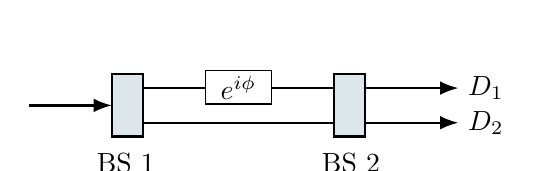
\begin{tikzpicture}[>=Latex,scale=.88]
\draw[->,thick](0,1)--(1.2,1);
\draw[thick,fill=accent!15](1.2,.55)rectangle(1.65,1.45);
\draw[thick](1.65,1.25)--(4.4,1.25);
\draw[thick](1.65,.75)--(4.4,.75);
\draw[thick,fill=accent!15](4.4,.55)rectangle(4.85,1.45);
\draw[->,thick](4.85,1.25)--(6.2,1.25);
\draw[->,thick](4.85,.75)--(6.2,.75);
\draw[fill=white](2.55,1.02)rectangle(3.5,1.5);
\node at (3.025,1.26){\(e^{i\phi}\)};
\node[below]at(1.4,.45){BS 1};
\node[below]at(4.65,.45){BS 2};
\node[right]at(6.2,1.25){\(D_1\)};
\node[right]at(6.2,.75){\(D_2\)};
\end{tikzpicture}
\end{center}

\subsection{Fisher information measures sensitivity}
The classical Fisher information for a
set of outcomes \(x\) is
\[
\boxed{F(\phi)=\sum_x
p(x|\phi)[\partial_\phi\ln p(x|\phi)]^2
=\sum_x\frac{(\partial_\phi p_x)^2}{p_x}.}
\]
A large \(F\) means a small phase change
strongly changes the outcome distribution.
For \(M\) independent measurements, the
classical Cram\'er--Rao bound is
\[
\operatorname{Var}(\tilde\phi)
\ge\frac{1}{MF(\phi)}
\]
for unbiased estimators under the usual
regularity assumptions.

\begin{worked}{Information in a single-photon interferometer}
For \(p_1=\cos^2(\phi/2)\),
\(p_2=\sin^2(\phi/2)\), differentiate:
\[
\partial_\phi p_1=-\tfrac12\sin\phi,\qquad
\partial_\phi p_2=+\tfrac12\sin\phi.
\]
Hence
\[
F=\frac{\sin^2\phi}{4}
\left[\frac1{\cos^2(\phi/2)}
+\frac1{\sin^2(\phi/2)}\right]
=\boxed{1},
\]
with the same continuous limit at endpoints.
The phase standard deviation cannot be
smaller than \(1/\sqrt M\) in this ideal
single-photon measurement model.
\end{worked}

\subsection{Quantum Fisher information}
The quantum Fisher information \(F_Q\)
is the largest information obtainable
by optimising over possible measurements.
For a pure probe encoded through
\(\ket{\psi_\phi}=e^{-i\phi G}\ket{\psi_0}\),
\[
\boxed{F_Q=4\operatorname{Var}_{\psi_0}(G).}
\]
An optical phase generated by photon number
has \(G=n\). For a coherent state
\(\operatorname{Var}(n)=\bar n\), so
\(F_Q=4\bar n\), giving the characteristic
shot-noise scaling
\(\Delta\phi\propto1/\sqrt{\bar n}\).
Different conventions for whether the
parameter is the phase on one arm or the
relative arm phase alter constant factors
in the generator, but not this scaling.

\subsection{How squeezing can help, and when it cannot}
A squeezed input can improve sensitivity
when its quiet quadrature matches the
noise relevant to the measurement.
In a gravitational-wave interferometer,
squeezed vacuum is often injected into
an otherwise unused port to reduce
measured quantum fluctuations.
However, \emph{one squeezed-coherent input
plus vacuum in the other port}, measured
by simple output-number difference at
a balanced operating phase, can still
give variance equal to total input
mean photon number. That specific
configuration does not automatically
beat shot-noise scaling at equal energy.

\begin{checkpoint}
When asked for precision, identify:
the encoded parameter, generator \(G\),
actual measurement outcomes, photon
resource, repetitions and operating
phase. QFI is an \emph{optimised bound};
a particular detector may not attain it.
\end{checkpoint}

\partmarking{III}{Atomic physics}
\unit{Hydrogenic atoms and radial wavefunctions}
\unitref{Week 8; 2023 Q2; Assignment 3 Q1; Assignment 4 Q3}
\subsection{The one-electron Schr\"odinger equation}
For an electron of reduced mass \(\mu\)
around a point nucleus of charge \(+Ze\),
\[
\left[-\frac{\hbar^2}{2\mu}\nabla^2
-\frac{Ze^2}{4\pi\epsilon_0r}\right]
\psi(\mathbf r)=E\psi(\mathbf r).
\]
The Coulomb potential depends only on
the radius \(r\), so angular momentum is
conserved. Separate variables into
\[
\boxed{\psi_{nlm}(\mathbf r)=R_{nl}(r)
Y_{lm}(\theta,\phi).}
\]
The spherical harmonics are eigenfunctions
of \(L^2,L_z\) with
\[
L^2Y_{lm}=\hbar^2l(l+1)Y_{lm},\qquad
L_zY_{lm}=\hbar mY_{lm}.
\]
The labels have allowed values
\(n=1,2,\ldots\), \(l=0,\ldots,n-1\),
\(m=-l,\ldots,l\).

\subsection{The centrifugal barrier}
Define \(u(r)=rR_{nl}(r)\).
Then the radial Schr\"odinger equation becomes
\[
\boxed{-\frac{\hbar^2}{2\mu}\frac{d^2u}{dr^2}
+\left[V(r)+\frac{\hbar^2l(l+1)}{2\mu r^2}\right]u
=Eu.}
\]
The term proportional to \(1/r^2\)
is the effective centrifugal barrier.
For \(l>0\), the radial wavefunction
is suppressed near the nucleus;
\(s\)-states with \(l=0\) penetrate it
much more strongly.
The normalisation can be written
\[
\int_0^\infty|R_{nl}|^2r^2dr
=\int_0^\infty|u_{nl}|^2dr=1.
\]
Switching from \(R\) to \(u\) changes the
\emph{measure} in every radial matrix element.

\subsection{Why hydrogen energies depend only on \(n\)}
The nonrelativistic Coulomb levels are
\[
\boxed{E_n=-\frac{\mu Z^2e^4}
{2(4\pi\epsilon_0)^2\hbar^2n^2}
\approx-13.6\,{\rm eV}\,
\frac{\mu}{m_e}\frac{Z^2}{n^2}.}
\]
The \(n\)-only degeneracy is a special
symmetry of the pure Coulomb potential.
Screening in a many-electron atom,
relativity, magnetic fields and finite
nuclear size lift different parts
of this degeneracy.

\begin{worked}{Most probable radius is not mean radius}
For hydrogen \(1s\),
\(\psi_{1s}=e^{-r/a_0}/\sqrt{\pi a_0^3}\).
The probability in a spherical shell
between \(r\) and \(r+dr\) is
\[
P(r)dr=4\pi r^2|\psi|^2dr
=\frac{4r^2}{a_0^3}e^{-2r/a_0}dr.
\]
Differentiate \(\ln P(r)\):
\(2/r-2/a_0=0\), so
\(\boxed{r_{\rm most\ probable}=a_0}\).
But
\[
\langle r\rangle=\frac4{a_0^3}
\int_0^\infty r^3e^{-2r/a_0}dr
=\boxed{3a_0/2}.
\]
The different answers are not contradictory:
one describes the peak of a distribution;
the other its average.
\end{worked}

\subsection{Finite nuclear size is a perturbation}
A nucleus has a finite radius and a spread-out
charge distribution. The point Coulomb potential
\(-Z/r\) is too singular near the origin.
For a uniform nuclear sphere of radius \(R\)
in atomic units,
\[
V_{\rm finite}(r)=
-\frac{Z}{2R}\left(3-\frac{r^2}{R^2}\right)
\quad(r<R).
\]
The perturbation is
\[
\Delta V=V_{\rm finite}-V_{\rm point}
=Z\left(\frac1r-\frac{3}{2R}
+\frac{r^2}{2R^3}\right).
\]
First-order perturbation theory gives
\[
\boxed{\Delta E_{nl}=\int_0^R
|R_{nl}(r)|^2r^2\Delta V(r)\,dr.}
\]
If \(R\) is small and the \(s\)-state
wavefunction is approximately constant
inside the nucleus, one obtains
\[
\boxed{\Delta E_{ns}\simeq
\frac{2Z^4R^2}{5n^3}\quad\text{(Hartree)}.}
\]
The positive shift makes the state less
strongly bound. It is particularly
large for orbitals with nonzero density
at the origin.

\subsection{How numerical radial solutions work}
For a screened or model potential \(V(r)\),
the radial equation is often discretised.
At grid spacing \(h\),
\[
u''(r_i)\approx
\frac{u(r_{i-1})-2u(r_i)+u(r_{i+1})}{h^2}.
\]
The Hamiltonian becomes a sparse
tridiagonal matrix. Diagonalising it
yields energies and radial eigenvectors.
Check normalisation, radial nodes and
stability as \(h\) decreases and
the outer boundary moves outward.
The sodium lifetime assignment uses
exactly this kind of numerical workflow.

\begin{checkpoint}
Hydrogenic \(n,l,m\) label wavefunctions,
not miniature classical orbits.
For a radial integral, always decide
whether you are using \(R(r)\) or
\(u(r)=rR(r)\) before writing the measure.
\end{checkpoint}

\unit{Many-electron atoms, configurations and term symbols}
\unitref{Week 8; Assignment 3 Q2; Assignment 4 Q1}
\subsection{Why the hydrogen formula stops working}
Two electrons repel each other. The
many-electron Hamiltonian has the form
\[
\boxed{H=\sum_i\left[\frac{p_i^2}{2m_e}
-\frac{Ze^2}{4\pi\epsilon_0r_i}\right]
+\sum_{i<j}\frac{e^2}{4\pi\epsilon_0r_{ij}}.}
\]
The last term depends on \emph{two}
electron positions, so we cannot solve
each electron independently as if the
other electrons were absent.
An approximate central potential describes
the nucleus screened by the electron cloud.
The one-electron orbitals are labelled
\(n,l\), but their energies are no longer
functions of \(n\) alone.

\subsection{Pauli exclusion and antisymmetric states}
Electrons have spin \(s=1/2\) and
are identical fermions. Interchanging
two electron labels must reverse
the \emph{total} wavefunction:
\[
\Psi(1,2)=-\Psi(2,1).
\]
A two-electron Slater determinant
automatically enforces this:
\[
\Psi_{ab}(1,2)=\frac1{\sqrt2}
[a(1)b(2)-b(1)a(2)].
\]
If \(a=b\), the determinant vanishes:
two electrons cannot occupy the
same spin-orbital.

\subsection{Direct repulsion and exchange}
Evaluate Coulomb repulsion
\(v_{12}=e^2/(4\pi\epsilon_0r_{12})\)
in a Slater determinant. Expanding
the bra and ket yields
\[
\boxed{\langle v_{12}\rangle=J_{ab}-K_{ab}},
\]
where
\[
J_{ab}=\iint\frac{|a(1)|^2|b(2)|^2}{r_{12}}\,
d1\,d2,
\]
\[
K_{ab}=\iint\frac{a^*(1)b(1)b^*(2)a(2)}
{r_{12}}\,d1\,d2
\]
in atomic units. The direct term resembles
ordinary Coulomb repulsion between densities.
The exchange term arises from the
antisymmetric \emph{wavefunction}.
It is not another classical force;
for orthogonal spin labels it vanishes.
Hartree--Fock finds orbitals self-consistently
so that direct and exchange contributions
enter the mean-field equations.

\subsection{How spectroscopic term notation works}
For light atoms with reasonably good
LS (Russell--Saunders) coupling, first
add the individual orbital momenta to
\(L\), individual electron spins to
\(S\), then couple \(L,S\) to total
electronic \(J\). Write
\[
\boxed{{}^{2S+1}L_J},\qquad
L=0,1,2,3,4\leftrightarrow S,P,D,F,G.
\]
For example, \({}^3F_2\) means
total spin \(S=1\) (triplet),
total orbital angular momentum \(L=3\)
and total electronic \(J=2\).
The allowed \(J\) values are
\(J=|L-S|,|L-S|+1,\ldots,L+S\).

\subsection{Equivalent electrons require extra care}
Two \(d\) electrons each have \(l=2\)
and two spin projections. There are
ten distinct spin-orbitals, hence
\[
\binom{10}{2}=45
\]
antisymmetric configurations.
Without Pauli restrictions, angular-momentum
addition would suggest \(L=0,1,2,3,4\),
\(S=0,1\). But the orbital-coupled
wavefunction has exchange phase
\((-1)^{2l-L}=(-1)^L\).
The spin singlet \(S=0\) is antisymmetric,
while triplet \(S=1\) is symmetric.
Thus only \emph{even \(L\), \(S=0\)}
or \emph{odd \(L\), \(S=1\)} survive:
\[
\boxed{{}^1S_0,\ {}^1D_2,\ {}^1G_4,\quad
{}^3P_{0,1,2},\ {}^3F_{2,3,4}.}
\]

\begin{worked}{Check that every \(d^2\) state is counted}
A term with total \(J\) has \(2J+1\)
magnetic substates. Sum:
\[
1+5+9+(1+3+5)+(5+7+9)=\boxed{45}.
\]
The count agrees with the Pauli
spin-orbital count \(\binom{10}{2}\).
Without this check we could easily
include forbidden LS terms or miss
part of an allowed multiplet.
\end{worked}

\subsection{Hund's rules and why they are only trends}
Within their usual domain, Hund's rules
favour (1) largest total \(S\), then
(2) largest \(L\) for that multiplicity,
then (3) smallest \(J\) in a
less-than-half-filled subshell.
For \(d^2\), this predicts
the ground level \({}^3F_2\).
However, these rules do \emph{not}
unambiguously order every excited term
of a real multi-electron atom.
Titanium's neutral \(3d^24s^2\)
configuration demonstrates the broad
agreement and exceptions when compared
with NIST experimental level data.

\begin{checkpoint}
The notation \({}^{2S+1}L_J\) is a
coupling scheme, not a claim that
electrons orbit independently.
First impose antisymmetry, then
enumerate LS terms, attach \(J\),
and check the total degeneracy.
\end{checkpoint}

\unit{Adding angular momenta, Clebsch--Gordan and 3-j symbols}
\unitref{Week 8; 2025 Q1; Atomic Assignment 4 Q1}
\subsection{What is being added?}
An electron has orbital angular momentum
\(\mathbf L\) and spin \(\mathbf S\);
an atom may have nuclear angular momentum
\(\mathbf I\). The sum of two angular
momentum vectors is again an angular
momentum operator:
\(\mathbf J=\mathbf J_1+\mathbf J_2\).
But a simultaneous eigenstate of
\(J_1^2,J_2^2,J^2,J_z\) is not generally
a product of separate \(J_{1z}\) and
\(J_{2z}\) eigenstates.

Angular momentum eigenvalues are
\[
J^2\ket{jm}=\hbar^2j(j+1)\ket{jm},
\qquad J_z\ket{jm}=\hbar m\ket{jm}.
\]
For \(j_1,j_2\), the allowed total \(j\) values are
\[
\boxed{j=|j_1-j_2|,\ |j_1-j_2|+1,\ldots,j_1+j_2.}
\]
The total projection is \(m=m_1+m_2\).
That is the \emph{angular-momentum addition rule}.

\subsection{What does a Clebsch--Gordan coefficient say?}
In the product basis,
\(\ket{j_1m_1}\ket{j_2m_2}\) describes
known projections of the two components.
In the coupled basis \(\ket{JM}\),
the magnitude of the \emph{total}
angular momentum is known.
The relation is a change of basis:
\[
\boxed{\ket{JM}=
\sum_{m_1m_2}
\braket{j_1m_1,j_2m_2}{JM}
\ket{j_1m_1}\ket{j_2m_2}.}
\]
The number in angle brackets is a
Clebsch--Gordan (CG) coefficient.
It is a probability \emph{amplitude}
for a particular uncoupled pair, not
a physical coupling energy or a probability by itself.

\begin{worked}{Two spin-\(\tfrac12\) particles from scratch}
Each particle has \(\ket\uparrow\) or
\(\ket\downarrow\). Addition allows
\(J=1\) (triplet) and \(J=0\) (singlet).
The coupled states are
\[
\begin{aligned}
\ket{1,1}&=\ket{\uparrow\uparrow},\\
\ket{1,0}&=\frac{\ket{\uparrow\downarrow}
+\ket{\downarrow\uparrow}}{\sqrt2},\\
\ket{1,-1}&=\ket{\downarrow\downarrow},\\
\ket{0,0}&=\frac{\ket{\uparrow\downarrow}
-\ket{\downarrow\uparrow}}{\sqrt2}.
\end{aligned}
\]
Thus
\(\langle\tfrac12,\tfrac12;
\tfrac12,-\tfrac12|1,0\rangle=1/\sqrt2\).
The same product basis component
has overlap \(1/\sqrt2\) with the singlet.
Triplet and singlet states are
orthogonal, and the four coupled
states span the same four-dimensional
Hilbert space as the four product states.
\end{worked}

\subsection{Why introduce a 3-j symbol?}
A Wigner 3-j symbol is a conventional
normalised version of a CG coefficient:
\[
\boxed{
\begin{pmatrix}j_1&j_2&J\\m_1&m_2&-M\end{pmatrix}
=\frac{(-1)^{j_1-j_2+M}}
{\sqrt{2J+1}}
\langle j_1m_1,j_2m_2|JM\rangle.}
\]
It is useful because its symmetry
properties make selection rules and
angular integrations compact.
Before calculating a value, test:
\[
|j_1-j_2|\le j_3\le j_1+j_2,\qquad
m_1+m_2+m_3=0,\qquad |m_i|\le j_i.
\]
If a condition fails, the symbol is zero.
This often answers a whole transition
question before numerical evaluation.

\begin{worked}{A concrete \(3j\) calculation}
Adding zero angular momentum to \(j=1\)
does nothing:
\[
\langle 0,0;1,0|1,0\rangle=1.
\]
Use the relation above with
\(j_1=0,j_2=1,J=1,M=0\):
\[
\begin{pmatrix}0&1&1\\0&0&0\end{pmatrix}
=\frac{(-1)^{0-1+0}}{\sqrt3}(1)
=\boxed{-\frac1{\sqrt3}}.
\]
There is no need to memorise the
full factorial formula for this special case.
For less obvious values, consult the
CG/3-j tables provided in the course
or use a symbolic-algebra program.
\end{worked}

\subsection{Wigner--Eckart: separate geometry from physics}
A spherical tensor operator \(T_q^{(k)}\)
has rank \(k\) and component \(q=-k,\ldots,k\).
Electric dipole is rank 1; electric
quadrupole is rank 2.
For a chosen reduced-element convention,
\[
\boxed{
\mel{j'm'}{T_q^{(k)}}{jm}
=(-1)^{j'-m'}
\begin{pmatrix}j'&k&j\\-m'&q&m\end{pmatrix}
\langle j'\Vert T^{(k)}\Vert j\rangle.}
\]
The 3-j symbol gives the allowed
\emph{geometry}, including the projection
condition \(m'=m+q\).
The reduced matrix element contains
the specific radial/atomic physics but
is independent of \(m,m',q\).
Two transitions within the same
multiplet can therefore have
different strengths entirely because
their 3-j coefficients differ.

\subsection{A transition example with \(J=0\to J'=1\)}
An E1 operator has \(k=1\). Begin
in \(J=0,m=0\). The triangle rule permits
\(J'=1\). If the light has tensor
component \(q=+1\), then \(m'=1\)
because \(m'=m+q\).
For \(q=0\), the only final projection is
\(m'=0\). In both cases the absolute
angular coefficient is \(1/\sqrt3\)
in the displayed Wigner--Eckart convention.
Whether the actual transition occurs
still depends on the \emph{reduced}
dipole element and parity.

\subsection{Why parity is an independent test}
Under spatial inversion,
\(\mathbf r\mapsto-\mathbf r\).
A dipole operator \(\mathbf d=-e\mathbf r\)
changes sign. If the initial and final
states have identical parity, the
integrand of \(\langle f|\mathbf d|i\rangle\)
is odd and the integral vanishes.
Therefore a nonzero 3-j symbol does
\emph{not} by itself guarantee E1 emission.

\begin{checkpoint}
Use the shortest sequence:
(1) determine total \(J\) and projection
possibilities; (2) test 3-j triangle and
magnetic-number rules; (3) check parity;
(4) only then evaluate a 3-j coefficient
and reduced atomic matrix element.
\end{checkpoint}

\unit{Fine structure, hyperfine structure and fields}
\unitref{Weeks 8--9; Assignment 3 Q4; 2025 Q1}
\subsection{Why one electronic configuration has many levels}
The central-field approximation produces
orbital energies but does not yet include
all small interactions. Electron spin--orbit
coupling links the orbital and spin
magnetic moments; the atomic nucleus has
its own spin and magnetic moment; external
electric and magnetic fields shift the levels.
These effects create fine, hyperfine,
Zeeman and Stark structures with
different typical energy scales.

\subsection{Fine structure from \(\mathbf L\cdot\mathbf S\)}
Suppose \(H_{\rm SO}=A_{\rm SO}\,
\mathbf L\cdot\mathbf S/\hbar^2\)
within an LS term. Since
\[
\mathbf J^2=(\mathbf L+\mathbf S)^2
=\mathbf L^2+\mathbf S^2+
2\mathbf L\cdot\mathbf S,
\]
the energy correction is
\[
\boxed{E_J^{\rm SO}=\frac{A_{\rm SO}}2
[J(J+1)-L(L+1)-S(S+1)].}
\]
This is more than a formula to remember:
it is simply the scalar product identity
for two angular momenta.

\begin{worked}{Split a \({}^3D\) term}
The term has \(S=1,L=2\), so
\(J=1,2,3\). With \(L(L+1)=6\) and
\(S(S+1)=2\),
\[
E_1=-3A_{\rm SO},\quad
E_2=-A_{\rm SO},\quad
E_3=2A_{\rm SO}.
\]
The degeneracies \(3+5+7=15\)
equal \((2L+1)(2S+1)=5\times3\).
The level intervals \(2A_{\rm SO}\)
and \(3A_{\rm SO}\) are not equally spaced.
\end{worked}

\subsection{Hyperfine structure couples electrons to the nucleus}
The nuclear spin \(\mathbf I\) combines
with electronic \(\mathbf J\) to form
\(\mathbf F=\mathbf I+\mathbf J\).
For magnetic-dipole hyperfine coupling,
\[
H_{\rm hfs}=\frac{A}{\hbar^2}\mathbf I\cdot\mathbf J,
\]
giving
\[
\boxed{E_F=\frac A2[
F(F+1)-I(I+1)-J(J+1)]},\quad
F=|I-J|,\ldots,I+J.
\]
The numerical sign of \(A\) matters:
the labels alone do not establish
which \(F\) has higher energy.
Electric quadrupole and higher-rank
nuclear hyperfine interactions are
possible only if the nuclear and
electronic tensor ranks allow them.

\begin{worked}{The 2025 exam hyperfine example}
Let \(I=5/2,J=1/2\).
Then \(F=2,3\).
Since \(I(I+1)=35/4\),
\(J(J+1)=3/4\),
\[
E_2=\frac A2(6-38/4)=
\boxed{-7A/4},
\quad
E_3=\frac A2(12-38/4)=
\boxed{5A/4}.
\]
Their separation is \(3|A|\).
The magnetic substate count
\((2F_1+1)+(2F_2+1)=5+7=12\)
agrees with \((2I+1)(2J+1)=6\times2\).
\end{worked}

\subsection{The weak magnetic-field regime}
A magnetic field interacts with atomic
magnetic moments. When hyperfine coupling
dominates the Zeeman energy,
\(F,m_F\) remain useful approximate
quantum numbers:
\[
\boxed{\Delta E_{Fm_F}\simeq
\mu_Bg_Fm_FB.}
\]
Neglecting the much smaller nuclear
magnetic contribution and for \(F>0\),
\[
g_F\simeq g_J
\frac{F(F+1)+J(J+1)-I(I+1)}
{2F(F+1)}.
\]
The electronic Land\'e factor for
\(g_L=1,g_S\simeq2\) is
\[
\boxed{g_J\simeq1+
\frac{J(J+1)+S(S+1)-L(L+1)}
{2J(J+1)}}.
\]
These factors arise from \emph{projecting}
electronic orbital/spin moments first
onto \(J\), then onto \(F\).

\subsection{The strong-field (Paschen--Back) regime}
When Zeeman energy exceeds hyperfine
coupling, nuclear and electronic
angular momenta approximately decouple.
The natural basis changes from
\(\ket{Fm_F}\) to \(\ket{Jm_J,Im_I}\).
To first order,
\[
E\simeq g_J\mu_Bm_JB+Am_Im_J
\]
if the nuclear Zeeman contribution is
neglected. The total state count stays
constant, but the interpretation
of the levels changes.
A fixed-\(F\) weak-field formula
must \emph{not} be extrapolated
to arbitrarily large \(B\).

\subsection{Electric fields: the Stark effect}
A static electric field \(\mathcal E\hat z\)
couples through \(-\mathbf d\cdot\boldsymbol{\mathcal E}\).
For a nondegenerate parity eigenstate
with no permanent electric dipole,
the first-order shift vanishes.
Second-order perturbation theory gives
\[
\boxed{\Delta E^{(2)}=-\frac12
\alpha(0)\mathcal E^2,\quad
\alpha(0)=2\sum_{n\ne i}
\frac{|\langle n|d_z|i\rangle|^2}{E_n-E_i}}.
\]
The polarisability measures how readily
the atom's electron cloud responds to
an applied field. For a hydrogenic \(1s\)
state a closure approximation using
\(E_n-E_1\approx E_2-E_1\) gives
\(\alpha_{\rm approx}=16/(3Z^4)\)
in atomic polarizability-volume units,
compared with the exact hydrogen value
\(9/2\) at \(Z=1\).

\begin{checkpoint}
Identify the relevant coupling hierarchy.
Fine structure: \(L+S\to J\).
Hyperfine: \(I+J\to F\).
Weak magnetic field: \(F,m_F\).
Strong magnetic field: \(m_I,m_J\).
Electric field: check parity before
applying Stark perturbation theory.
\end{checkpoint}

\partmarking{IV}{Applications of atomic physics}
\unit{Atomic spectroscopy, multipoles and radiative lifetimes}
\unitref{Week 9; Week 10; Assignment 4 Q3}
\subsection{Absorption and emission connect energy levels}
An atom absorbs light when an electromagnetic
mode drives a transition between its
quantum energy eigenstates. Energy
conservation fixes
\[
\hbar\omega_{if}=E_i-E_f,\quad
\nu=\frac{E_i-E_f}{h},\quad
\lambda=\frac{hc}{E_i-E_f}.
\]
A positive energy difference alone does
not guarantee a transition:
the light--matter interaction operator
must have a nonzero matrix element
between the two states.

\subsection{Electric dipole coupling}
The leading long-wavelength interaction
is \(H_{\rm int}=-\mathbf d\cdot\mathbf E\),
where the electron dipole is \(\mathbf d=-e\mathbf r\).
The transition amplitude contains
\[
\mathcal M_{fi}\propto
\bra f\mathbf d\cdot\boldsymbol\epsilon\ket i.
\]
This separates into radial and angular
factors when orbitals are expressed as
\(R_{nl}(r)Y_{lm}(\theta,\phi)\).
For an electric dipole the radial integral is
\[
\boxed{\int_0^\infty
R_f^*(r)R_i(r)\,r^3dr}
\]
or, using \(u=rR\),
\(\int u_f^*(r)\,r\,u_i(r)dr\).
The power \(r^3\) combines the
\(r^2dr\) volume measure with
the additional \(r\) from the dipole.

\subsection{Multipole rank and parity rules}
An electric multipole \(Ek\)
is a rank-\(k\) spherical tensor
of parity \((-1)^k\);
a magnetic multipole \(Mk\)
has parity \((-1)^{k+1}\).
For total angular momenta \(J,J'\),
the geometric rule is
\[
\boxed{|J-J'|\le k\le J+J',\qquad
m'=m+q,\quad |q|\le k.}
\]
For the most common transitions:
\[
\begin{array}{l|l|l}
&\text{Parity}&\text{Common }J\text{ rules}\\\hline
E1\ (k=1)&\text{changes}&
\Delta J=0,\pm1,\;0\nleftrightarrow0\\
M1\ (k=1)&\text{same}&
\Delta J=0,\pm1,\;0\nleftrightarrow0\\
E2\ (k=2)&\text{same}&
|\Delta J|\le2,\ J+J'\ge2
\end{array}
\]
The usual E1 orbital rule for one electron
is \(\Delta l=\pm1\).
For E2 the single-electron orbital rules
are \(\Delta l=0,\pm2\), subject to triangle
conditions. Thus \(s\leftrightarrow d\)
can be E2, but \(s\leftrightarrow p\)
is not E2 because parity changes.
Additional approximate LS coupling rules,
such as \(\Delta S=0\) for electric-dipole
transitions, may be softened by spin--orbit
mixing. A weak intercombination line can
therefore exist even if it is forbidden
in ideal LS coupling.

\begin{worked}{Which sodium transitions can radiate by E1?}
The valence-orbital transitions
\(3p\to3s\), \(4s\to3p\)
and \(3d\to3p\) all have
\(\Delta l=\pm1\), so their
orbital E1 matrix elements may
be nonzero. But \(3d\to3s\)
has \(\Delta l=-2\) and is E1 forbidden.
Always check \emph{downward energy ordering}
for spontaneous emission: an angularly
allowed upward transition is absorption,
not spontaneous decay from a lower level.
\end{worked}

\subsection{Why some states decay quickly}
An excited atom couples to vacuum
electromagnetic modes and can
spontaneously emit a photon. For an
E1 transition between appropriately
specified states,
\[
\boxed{A_{if}=
\frac{\omega_{if}^3}{3\pi\epsilon_0\hbar c^3}
|\bra f\mathbf d\ket i|^2,}
\]
where the displayed vector dipole
strength and sublevel/polarisation
summations must be handled consistently.
The strong \(\omega^3\) dependence means
larger energy gaps generally radiate
faster for comparable matrix elements.
A forbidden E1 line may instead decay
by much weaker M1/E2 channels,
making it useful for long-lived
clock or metastable states.

\subsection{Lifetime and branching ratios}
If an excited state can decay into
several lower states,
\[
\boxed{\Gamma_i=\sum_{f<i}A_{if},\quad
\tau_i=\Gamma_i^{-1},\quad
b_{if}=\frac{A_{if}}{\Gamma_i}.}
\]
Do \emph{not} use the inverse
of just one \(A\) if multiple
important decay channels exist.
In quantum optics \(\Gamma_i\)
is a population decay rate with units
\(\mathrm{s}^{-1}\); a natural
linewidth in angular-frequency units
is of order \(\Gamma_i\).

\begin{worked}{A transition-rate calculation with a stated dipole}
For a \emph{hypothetical} 589 nm line with
\(|\mathbf d|=2ea_0\) and no other
downward channels,
\[
\omega=\frac{2\pi c}{589\,\mathrm{nm}},
\quad
A=\frac{\omega^3(2ea_0)^2}
{3\pi\epsilon_0\hbar c^3}.
\]
This gives a rate of order
\(4\times10^7\ \mathrm{s}^{-1}\)
and a lifetime of order
\(25\) ns. It is an illustration
of using the formula, \emph{not}
a claim about a measured Na lifetime.
For actual sodium, compute the
wavefunction-derived matrix elements
and sum all allowed channels.
\end{worked}

\subsection{Einstein coefficients and induced processes}
An incident radiation field can
stimulate both absorption and emission.
Einstein's \(A\) coefficient describes
spontaneous decay; the \(B\) coefficients
describe rates proportional to the
radiation energy density.
Their detailed-balance relations explain
thermal equilibrium radiation and
underlie laser gain calculations.
A large population inversion makes
stimulated emission dominate absorption
at the selected lasing transition.

\begin{checkpoint}
A complete transition question requires
\emph{energy}, \emph{tensor rank},
\emph{angular-momentum triangle},
\emph{parity}, and a \emph{reduced
matrix element}. A lifetime then needs
all allowed downward branches.
\end{checkpoint}

\unit{Driving, cooling and trapping atoms with lasers}
\unitref{Week 10; 2025 Q2; Zeeman slower tutorial}
\subsection{A laser couples two atomic levels}
Near an isolated optical transition,
model the atom with \(\ket g,\ket e\).
A classical electric field
\(\mathbf E(t)=\mathbf E_0\cos(\omega_Lt)\)
couples through \(-\mathbf d\cdot\mathbf E(t)\).
The \emph{Rabi frequency} measures
interaction strength:
\[
\boxed{\Omega=\frac{|\bra e\mathbf d\cdot
\mathbf E_0\ket g|}{\hbar}}
\]
with factors of 2 depending on whether
\(E_0\) denotes the full real-field
amplitude or its positive-frequency
part. State the convention in a
pulse-timing problem.
In a rotating frame and under
the rotating-wave approximation,
a convenient effective Hamiltonian is
\[
H_{\rm rot}=\frac{\hbar}2
\begin{pmatrix}-\Delta&\Omega\\
\Omega&\Delta\end{pmatrix},
\quad
\Delta=\omega_L-\omega_{eg}.
\]
The generalised Rabi frequency is
\(\Omega_{\rm eff}=\sqrt{\Omega^2+\Delta^2}\).

\subsection{Pulse area, pi and pi-over-two pulses}
For a resonant pulse with constant
coupling phase and time-dependent
amplitude \(\Omega(t)\),
the pulse area is
\(\Theta=\int\Omega(t)dt\).
An atom starting in \(\ket g\) has
\[
\boxed{P_e=\sin^2(\Theta/2).}
\]
A \(\pi\)-pulse transfers all population
to the excited state in the ideal
lossless model; a \(\pi/2\)-pulse
creates an equal-amplitude superposition.
Detuning prevents perfect inversion for
a constant-frequency rectangular pulse,
because the largest excited probability is
\(\Omega^2/(\Omega^2+\Delta^2)\).

\subsection{Why light can exert a force}
A photon carries momentum \(\hbar\mathbf k\).
Absorption transfers this directed momentum
to an atom. Spontaneous photons are emitted
in different directions, so their average
momentum along a fixed axis may vanish,
though their variance gives recoil heating.
For a driven two-level atom with excited-state
decay rate \(\Gamma\), a common steady-state
scattering rate is
\[
\boxed{R_{\rm sc}=\frac{\Gamma}{2}
\frac{s}{1+s+(2\Delta/\Gamma)^2}},
\qquad s=I/I_{\rm sat}.
\]
At high saturation on resonance,
\(R_{\rm sc}\to\Gamma/2\), giving
\[
\boxed{F_{\max}=\hbar k\Gamma/2,\qquad
a_{\max}=F_{\max}/M.}
\]
There is a trade-off: fast-scattering
broad transitions give strong slowing
forces but generally higher Doppler
cooling limits than narrow lines.

\subsection{Optical molasses and the Doppler shift}
An atom moving toward one of two
counter-propagating red-detuned beams
sees that beam Doppler-shifted
closer to resonance. It absorbs
more photons from the direction
opposing its motion, creating a
damping force near rest,
\(F\simeq-\beta v\).
In a simple two-level Doppler
cooling model, the minimum temperature is
\[
\boxed{T_D=\frac{\hbar\Gamma}{2k_B}
=\frac{\hbar}{2k_B\tau}},
\]
where \(\tau=1/\Gamma\).
The temperature comes from balancing
velocity damping against random
photon-recoil diffusion; the kinetic
energy never falls to exactly zero.

\subsection{A Zeeman slower follows changing velocity}
A fast atomic beam has a large Doppler
shift, which changes as atoms slow.
A position-dependent magnetic field
Zeeman-shifts the atomic transition
to maintain resonance with the
counter-propagating laser.
If the designed deceleration is constant,
\[
v(z)=\sqrt{v_0^2-2az},
\quad L=\frac{v_0^2}{2a},
\]
and, for a suitable sign convention,
the resonance field has the shape
\[
\boxed{B(z)=B_{\rm offset}
+B_0\sqrt{1-z/L}.}
\]
This is the origin of the characteristic
square-root slower profile, not merely
a curve fitted to experimental data.
An arbitrary field that reaches zero
need not slow atoms successfully:
the corresponding resonant velocity
must be dynamically followable.
Specifically,
\[
\boxed{a_{\rm req}(z)=
-v_{\rm res}(z)\frac{dv_{\rm res}}{dz}}
\]
must stay within the available scattering
acceleration and capture linewidth.

\begin{worked}{Estimate ytterbium stopping distance}
For the 2025 exam data,
\(M=1.73\times10^{-25}\,\mathrm{kg}\),
\(T=300\,\mathrm{K}\),
\(\lambda=399\,\mathrm{nm}\),
\(\tau=5.5\,\mathrm{ns}\),
choose the 3D rms speed
\(v_0=\sqrt{3k_BT/M}\approx268\,\mathrm{m/s}\).
At half the maximum scattering force,
\[
a=\frac{h}{4M\lambda\tau}
\approx4.36\times10^5\,\mathrm{m/s^2}.
\]
Hence
\[
L=\frac{v_0^2}{2a}\approx8.23\,\mathrm{cm},
\qquad
N_\gamma=\frac{Mv_0\lambda}{h}
\approx2.79\times10^4.
\]
The Doppler limit from this linewidth
is \(T_D\approx0.694\,\mathrm{mK}\).
The thermal speed convention affects
the stopping distance; state it explicitly.
\end{worked}

\subsection{Magneto-optical traps and selection rules}
A magneto-optical trap (MOT) uses
opposing red-detuned laser beams
with suitable circular polarisations
and a magnetic-field gradient.
Position-dependent Zeeman shifts
make one opposing beam more resonant,
producing a restoring force, while the
Doppler effect supplies damping.
Polarisation selection rules connect
light to atomic magnetic substates:
\(\pi\)-polarised light has \(\Delta m=0\);
\(\sigma^\pm\) components have
\(\Delta m=\pm1\), for a consistent
quantisation axis and photon helicity.
Optical pumping can redistribute
population among those substates.

\begin{checkpoint}
Rabi oscillations describe coherent drive.
Spontaneous scattering describes dissipative
momentum kicks. Doppler molasses damps
velocity; a MOT also restores position.
Zeeman slowing maintains resonance
while the beam loses speed.
\end{checkpoint}

\unit{Atoms as tests of parity and time-reversal symmetry}
\unitref{Week 12; atomic parity violation and EDM lectures}
\subsection{Why symmetry is a practical experimental tool}
An atomic experiment can be sensitive to
tiny interactions because ordinary
electromagnetic theory predicts that
certain transitions or energy shifts
should be \emph{zero} by symmetry.
If a supposedly forbidden signal
appears in a controlled measurement,
we investigate whether an interaction
absent from the simpler Hamiltonian
has broken that symmetry.
This motivates atomic tests of the
weak interaction, parity violation
and intrinsic electric dipole moments.

\subsection{What parity means}
A parity transformation inverts the
spatial coordinates:
\(\mathbf r\mapsto-\mathbf r\).
For a central potential, the orbital
wavefunctions have definite parity:
\[
P\ket{nlm}=(-1)^l\ket{nlm}.
\]
Thus \(s,d,g\) orbitals are even;
\(p,f\) orbitals are odd.
The electric dipole operator
\(\mathbf d=-e\mathbf r\)
is itself odd under parity.
If initial and final states have
the \emph{same} parity,
\[
\bra f\mathbf d\ket i
=-\bra f\mathbf d\ket i=0
\]
in a parity-conserving model.
This explains the E1 parity selection
rule without memorising a table.

\subsection{How the weak interaction changes the conclusion}
The electromagnetic Hamiltonian of
an atom approximately respects parity,
but the neutral-current weak
interaction contains parity-violating
electron--nucleus terms. Schematically,
\[
H=H_{\rm EM}+H_W,
\quad P H_WP^{-1}\ne H_W.
\]
First-order perturbation theory shows
that an originally definite-parity
state \(\ket i\) acquires admixtures
of opposite-parity states:
\[
\boxed{\ket{\tilde i}\approx\ket i+
\sum_{n\ne i}\ket n
\frac{\bra nH_W\ket i}{E_i-E_n}.}
\]
These admixtures can generate an
otherwise forbidden E1 amplitude
between same-parity levels.

\begin{worked}{Derive a weakly allowed E1 line}
Let \(\ket i,\ket f\) have the same
unperturbed parity and \(\ket n\)
the opposite parity. If only the
initial-state admixture matters,
\[
\ket{\tilde i}=\ket i+\epsilon\ket n,
\quad
\epsilon=\frac{\bra nH_W\ket i}{E_i-E_n}.
\]
Then
\[
\bra f d\ket{\tilde i}
=\underbrace{\bra f d\ket i}_{0}
+\epsilon\bra f d\ket n
=\boxed{\epsilon\bra f d\ket n}.
\]
A small mixing coefficient \(10^{-8}\)
multiplied by an allowed atomic dipole
of order \(ea_0\) gives a
\(10^{-8}ea_0\) amplitude.
In a full calculation, both initial
and final states can be mixed, and
one sums over many intermediate states.
\end{worked}

\subsection{Nuclear weak charge}
One widely discussed contribution
to atomic parity violation is
controlled by a nuclear weak charge,
with tree-level approximate form
\[
\boxed{Q_W\simeq-N+Z(1-4\sin^2\theta_W),}
\]
where \(N,Z\) are neutron and proton
numbers. Electroweak radiative
corrections and nuclear-structure
effects matter in precision work.
The measured parity-violating amplitude
also depends strongly on the atomic
electronic wavefunctions, so comparing
experiment with the Standard Model
requires accurate atomic many-body
theory, not just the weak charge.

\subsection{What is an intrinsic electric dipole moment?}
An electric dipole \(\mathbf d\) changes
sign under parity, while an axial
angular momentum \(\mathbf J\) does not.
A permanent \(\mathbf d\) aligned with
a particle's spin therefore violates
parity. Under time reversal,
spin changes direction but the electric
dipole does not, so such an intrinsic
EDM also violates time reversal.
The interaction energy is
\[
\boxed{H_{\rm EDM}=-\mathbf d\cdot
\boldsymbol{\mathcal E}.}
\]
A spin-precession experiment compares
frequencies for opposite electric-field
directions. A genuine EDM contribution
reverses sign with the electric field,
while carefully chosen combinations
of measurements reject common magnetic
and instrumental backgrounds.

\subsection{Schiff screening and experimental enhancement}
In a simple neutral atom of pointlike,
nonrelativistic Coulomb-interacting
constituents, internal fields screen
a uniformly applied static electric
field at the nucleus. This is the
basis of Schiff's theorem.
Finite nuclear size, relativistic
electron motion and molecular
polarisation circumvent its ideal
assumptions and can make EDM
measurements extremely sensitive.
Heavy atoms and polar molecules
are particularly useful because
their electronic and nuclear
structure can amplify some
symmetry-violating effects.

\subsection{Why this belongs in atomic physics}
The experimental quantity is a tiny
frequency shift or transition amplitude.
To predict it, one still needs the
atomic orbitals, good angular-momentum
coupling, selection rules, perturbation
theory and matrix elements developed
earlier in this mini-text.
A precision experiment turns those
familiar mathematical tools into a
test of fundamental interactions.

\begin{checkpoint}
Parity selection rules forbid amplitudes
\emph{only if} the Hamiltonian respects
parity and the basis states have definite
parity. A weak mixing interaction changes
the state and may open a previously
vanishing transition.
\end{checkpoint}

\unit{Atomic clocks and precision spectroscopy}
\unitref{Week 13; 2025 Q1; atomic applications}
\subsection{What makes an atom a clock?}
A clock is an oscillator whose phase
can be compared against a reference.
An atomic transition provides a frequency
associated with an exceptionally stable
energy difference:
\[
\boxed{\nu_0=\frac{E_{\rm upper}-E_{\rm lower}}{h}.}
\]
A laser or microwave oscillator is steered
to keep it on resonance with this
frequency. The atom does not generate
the counted electrical clock pulses
by itself: an interrogation sequence
and feedback system are needed.

\subsection{The caesium definition of the SI second}
The unperturbed ground-state hyperfine
transition of \(^{133}\mathrm{Cs}\) defines
the second, with frequency
\[
\boxed{\nu_{\rm Cs}=9\,192\,631\,770\ \mathrm{Hz}.}
\]
Caesium's valence ground term is
\(6s\,{}^2S_{1/2}\), so \(J=1/2\),
while the nuclear spin is \(I=7/2\).
Hyperfine coupling gives \(F=3,4\).
The clock transition is the
\[
\boxed{\ket{F=3,m_F=0}
\longleftrightarrow\ket{F=4,m_F=0}}
\]
transition. The choice \(m_F=0\) makes
the first-order Zeeman shift vanish
near zero field, reducing a major
source of frequency error.

\begin{worked}{Compute the caesium hyperfine interval}
With \(I=7/2,J=1/2\),
\(I(I+1)=63/4\) and \(J(J+1)=3/4\).
The magnetic-dipole hyperfine energy is
\[
E_F=\frac A2
[F(F+1)-I(I+1)-J(J+1)].
\]
Substitute \(F=3,4\):
\[
E_3=\frac A2(12-66/4)
=-\frac{9A}{4},\qquad
E_4=\frac A2(20-66/4)
=\frac{7A}{4}.
\]
Therefore \(E_4-E_3=4A\), so
\[
\boxed{A/h=\nu_{\rm Cs}/4
=2.2981579425\ \mathrm{GHz}.}
\]
The degeneracy check is
\(7+9=16=(2I+1)(2J+1)\).
\end{worked}

\subsection{Ramsey spectroscopy: letting phase accumulate}
In a Ramsey experiment a first
\(\pi/2\) pulse prepares an equal
superposition of clock states.
The atomic components then acquire
a relative phase during free evolution
for time \(T\). A second \(\pi/2\)
pulse converts that phase into
population. In the idealised
two-level model, the excited
population oscillates with detuning:
\[
P_e\sim\tfrac12[1+\cos(\Delta T+\phi_0)].
\]
The fringe width scales approximately
as \(1/T\). Long coherent interrogation
therefore permits a narrow frequency
discriminator, provided the atom
and the oscillator stay coherent.

\subsection{Why optical clocks can do better}
The quality factor of a spectral
reference is
\[
\boxed{Q=\frac{\nu_0}{\Delta\nu}}.
\]
A high carrier frequency and narrow
linewidth can yield a very high \(Q\).
For example, strontium optical clocks
use a transition near \(429\) THz,
vastly higher than the \(9.19\) GHz
caesium hyperfine carrier.
Optical clocks usually use specially
chosen metastable, narrow transitions
rather than bright, rapidly
decaying laser-cooling lines.

\subsection{Trapping without shifting the clock}
An optical lattice localises atoms,
reducing motional Doppler effects.
However, trapping light also shifts
atomic energy levels through the
AC Stark effect. At a
\emph{magic wavelength}, the
differential light shift of the
two clock states is approximately
zero, permitting confinement
without substantially shifting
the measured transition frequency.

\subsection{Stability and accuracy are different}
Stability describes the scatter
of clock frequency measurements
over an averaging time; accuracy
describes how closely the corrected
frequency matches the unperturbed
atomic reference. Quantum projection
noise, technical oscillator noise
and finite atom number affect
stability. Zeeman/Stark shifts,
black-body radiation, collisions
and gravitational redshift are
among the corrections important
for accuracy. A clock can be
very stable yet systematically wrong.

\subsection{Why clocks are physics experiments}
Comparing clocks based on different
species or transitions provides tests
of relativity and searches for
changes in fundamental constants.
Relativistic gravitational redshift
means clocks at different gravitational
potentials tick at measurably different
rates. Precise atomic spectroscopy
therefore connects quantum
structure to timekeeping, geodesy
and fundamental physics.

\begin{checkpoint}
A clock should have a long-lived,
narrow transition and be insensitive
to external perturbations.
The atomic transition, interrogation
sequence, local oscillator, feedback
and systematic corrections all
determine clock performance.
\end{checkpoint}

\partmarking{Appendices}{Mathematical toolkit and exam navigation}
\unit{A practical mathematical toolkit}
\unitref{Common methods across all four course parts}
\subsection{Expectation values in an eigenbasis}
Suppose \(\ket\psi=\sum_nc_n\ket n\),
where \(\ket n\) are eigenstates of an
observable \(A\) with eigenvalues \(a_n\).
Then
\[
\langle A\rangle=\sum_n|c_n|^2a_n,\quad
(\Delta A)^2=\sum_n|c_n|^2a_n^2
-\left(\sum_n|c_n|^2a_n\right)^2.
\]
The \emph{probabilities} are \(|c_n|^2\),
not \(c_n\). For operators not diagonal
in this basis, retain cross terms
\(c_m^*c_n\bra mA\ket n\).

\subsection{Commutators and transformations}
For Heisenberg evolution
\(\dot O=(i/\hbar)[H,O]\).
If \(H\) is a two-level Hamiltonian
\(H=(\hbar\Omega/2)\sigma_x\),
\[
U(t)=e^{-i\Omega t\sigma_x/2}
=I\cos(\Omega t/2)
-i\sigma_x\sin(\Omega t/2),
\]
because \(\sigma_x^2=I\).
For field displacement
\(D=e^{\alpha a^\dagger-\alpha^*a}\),
the identity \(D^\dagger aD=a+\alpha\)
follows by truncating the nested
commutator expansion after one step.

\subsection{Useful sums and integrals}
The geometric series for \(|q|<1\) is
\(\sum_{n=0}^\infty q^n=(1-q)^{-1}\).
Differentiate with respect to \(q\) to obtain
\[
\sum_{n=0}^\infty nq^n=\frac{q}{(1-q)^2},\quad
\sum_{n=0}^\infty n^2q^n
=\frac{q(1+q)}{(1-q)^3}.
\]
For \(\beta>0\) and integer \(m\ge0\),
\[
\boxed{\int_0^\infty r^me^{-\beta r}dr
=\frac{m!}{\beta^{m+1}}.}
\]
These formulas appear in thermal
photon statistics and hydrogen radial
expectation calculations.

\subsection{Perturbation theory}
For \(H=H_0+\lambda V\) and a
nondegenerate unperturbed state \(\ket i\),
\[
E_i^{(1)}=\bra iV\ket i,\qquad
E_i^{(2)}=
\sum_{n\ne i}\frac{|\bra nV\ket i|^2}
{E_i^{(0)}-E_n^{(0)}}.
\]
A first-order correction to the
\emph{state} is
\[
\ket{i^{(1)}}=
\sum_{n\ne i}\ket n
\frac{\bra nV\ket i}{E_i^{(0)}-E_n^{(0)}}.
\]
Use the energy formula for a
finite-nucleus or Stark \emph{shift};
use the state-mixing formula to
explain how weak parity violation
creates a forbidden transition.
For degenerate levels, first
diagonalise the perturbation in
the degenerate subspace.

\subsection{Fourier transforms of differential equations}
With the convention
\(\tilde f(\omega)=\int f(t)e^{-i\omega t}dt\),
\(\widetilde{\dot f}=i\omega\tilde f\).
Hence
\[
\dot a=-\lambda a+f(t)
\quad\Longrightarrow\quad
\boxed{\tilde a(\omega)=
\frac{\tilde f(\omega)}{\lambda+i\omega}}.
\]
A cavity susceptibility is an
instance of this elementary
linear-response formula.
The real damping rate appears
in the denominator together
with frequency detuning.

\subsection{Normalisation of conditional quantum states}
A detected branch is generally
\(\tilde\rho=K\rho K^\dagger\).
Keep its trace as the success
probability \(p=\operatorname{Tr}\tilde\rho\)
and only then write \(\rho_{\rm cond}=\tilde\rho/p\).
It is mathematically invalid to
normalise individual terms before
adding coherent amplitudes or
to sum conditional probabilities
without their branch weights.

\begin{worked}{A quick selection-rule test}
Suppose a putative E2 transition goes
from \(J=0\) to \(J'=1\).
E2 has tensor rank \(k=2\).
The triangle rule requires
\[
|0-1|\le2\le0+1,
\]
which fails at the right-hand inequality.
Therefore the rank-2 matrix element
vanishes before any radial integral
is evaluated. A parity check is
still needed for other pairs
that pass the triangle rule.
\end{worked}

\begin{checkpoint}
Often the difficult part is recognising
the \emph{right representation}.
Fock expansions for photon counts;
quadratures for homodyne/squeezing;
Kraus operators for channels;
small angular-momentum blocks for
atomic splittings; reduced matrix
elements for spectral transitions.
\end{checkpoint}

\unit{Question-type atlas, glossary and further practice}
\unitref{All tutorials, assignments and 2023--2025 examinations}
\subsection{Recognise a question before reaching for a formula}
The same few strategies recur throughout this course.
Use the table below to find the relevant teaching chapter
and then consult the longer worked-solutions booklets.
\begin{tabularx}{\linewidth}{@{}p{40mm}X@{}}
\toprule
\textbf{If the question asks about\ldots}&
\textbf{Start by doing this}\\\midrule
Coherent / thermal number counts&
Expand in \(\ket n\), form \(P_n\), evaluate
mean and factorial moments (Chapters 1--2)\\
HOM or photonic circuits&
Transform \emph{creation} operators and
normalise Fock states (Chapter 3)\\
Quadratures / squeezing&
State \([x,p]=2i\); compute means and
covariance, then apply the noise model (4--5)\\
Bell protocols and QKD&
Write the actual input state, gates,
measurement branches and sifted conditions (6--7)\\
Optical loss / postselection&
Include an environmental mode, trace or
project and normalise correctly (8--10)\\
Langevin cavity&
Commute Hamiltonian, Fourier transform and
apply the input--output boundary relation (9)\\
Atom--cavity coupling&
Choose conserved-excitation basis and
diagonalise a small block (11)\\
Quantum metrology&
Identify parameter generator and actual
measurement probabilities (12)\\
Hydrogen / nuclear size&
Separate \(R(r)Y_{lm}\); verify the radial
measure and use perturbation theory (13)\\
Configurations / LS terms&
Enforce antisymmetry; couple \(L,S,J\);
check the total state count (14)\\
3-j / transition amplitude&
Check triangle and \(m\) sums, then
Wigner--Eckart and parity (15,17)\\
Fine / hyperfine / Zeeman&
Choose \(L,S,J,I,F\), identify weak- or
strong-field basis, compute splitting (16)\\
Lifetime / multipoles&
Select allowed tensor rank and parity,
calculate dipole, sum all downward \(A\)'s (17)\\
Rabi pulse / laser cooling&
Distinguish coherent pulse area from
dissipative scattering force (18)\\
Atomic PV / EDM&
Find the symmetry-forbidden leading term,
then perturbatively mix states (19)\\
Cesium / optical clock&
Calculate hyperfine reference,
identify field-insensitive sublevels
and systematic shifts (20)\\
\bottomrule
\end{tabularx}

\subsection{Frequently confused concepts}
\textbf{Probability amplitude vs probability:}
a quantum state uses complex amplitudes;
only their modulus squared gives a probability.

\textbf{Coherent state vs pure state:}
a coherent state is one particular
pure oscillator state; many other
pure states are nonclassical.

\textbf{Mode overlap vs optical power:}
photon interference visibility depends
on mode indistinguishability, not just intensity.

\textbf{Relative phase vs global phase:}
a global factor \(e^{i\phi}\ket\psi\)
does not change measurement results,
but a relative phase between components does.

\textbf{Kraus channel vs conditional outcome:}
summed branches are trace preserving;
one selected detector outcome must
be renormalised and assigned a success probability.

\textbf{Angular momentum \(J\) vs term \(L,S\):}
total electronic \(J\) is the vector sum
of already coupled electronic orbital and spin moments.
Hyperfine \(F\) then adds nuclear \(I\).

\textbf{Allowed angular transition vs nonzero line strength:}
a 3-j symbol can pass selection rules
while the reduced atomic matrix element vanishes.

\textbf{Natural linewidth vs laser detuning:}
linewidth arises from decay/decoherence;
detuning is the frequency mismatch
between laser and atomic resonance.

\textbf{Clock accuracy vs stability:}
accuracy concerns systematic offset;
stability concerns fluctuations over averaging time.

\subsection{Physical constants and units that recur}
\[
\begin{array}{@{}ll@{}}
\hbar=h/(2\pi)&\text{reduced Planck constant}\\
a_0=5.29177\times10^{-11}\,\mathrm m&
\text{Bohr radius}\\
1E_h=27.2114\,\mathrm{eV}&\text{Hartree energy}\\
1E_h/(hc)=219474.63\,\mathrm{cm}^{-1}&
\text{atomic spectroscopy}\\
t_{\rm au}=2.418884\times10^{-17}\,\mathrm s&
\text{atomic unit of time}\\
\mu_B=e\hbar/(2m_e)&\text{Bohr magneton}\\
\alpha_{\rm fs}\simeq1/137.036&
\text{fine-structure constant}
\end{array}
\]
When a problem switches between wavelength,
wavenumber, frequency and angular frequency,
write each definition explicitly:
\[
\tilde\nu=1/\lambda,\quad
\nu=c/\lambda,\quad
\omega=2\pi\nu,\quad E=h\nu=\hbar\omega.
\]
The factors of \(2\pi\) are particularly
important in linewidth and Rabi calculations.

\subsection{Where to practise each technique}
The repository companion booklets are designed
to work together:
\begin{enumerate}
\item The \emph{15-page Course Overview} is the
fast exam-day map of key physical results.
\item The \emph{Worked Examples} booklet provides
twenty carefully selected full calculations.
\item The \emph{Assignment Solutions} booklet
develops derivations and numerical methods
associated with four assignment sheets.
\item The \emph{2023--2025 Past Exam Solutions}
booklet covers twelve full exam questions.
\end{enumerate}
In revision, read a mini-text chapter
and try the associated problem \emph{before}
looking at its worked solution.
List any remaining conceptual difficulty
in the repository's mistakes-and-gaps notes.
\begin{checkpoint}
An exam solution is strongest when it
connects a choice of model, a governing
operator, a calculation, a limiting-case
check and a physical interpretation.
\end{checkpoint}

\end{document}
